\section{Simulation Results}
The simulation results in this chapter will consist of two types. The first type will be where the terrain does provide positive $F_{net,DB}$ values across a domain of $i$ values but the traction control architecture has too large of an error in $\hat{i}_{pk}$ to maintain tractor mobility. Here, the winch control mode will activate so as to allow the tractor to maintain mobility where it normally would not. This type of simulation result will be conducted for the red tractor from the previous chapter where the tractor lost mobility using only the traction control mode. The second set of simulation results will show four tractors traversing different soft terrains where $F_{net,DB}$ is negative for all slip values $i$. Under these operating conditions, the tractor must be equipped with a winch to maintain mobility. 

In Ch. \ref{ch:TCM}, results showed that all 5 tractors except the red one was able to maintain mobility across 100 meter soft terrain stretch. However, the red tractor did traverse $\sim$53 of the 100 meters. Now, the red tractor will use its winch to traverse the remaining $\sim$47 meters and beyond. Furthermore, it should be noted that the combined capability of the traction control mode and the winch control mode allows for terrain traversal without having to forfeit cable across the entire 100 meters to minimize the amount of cable length required.

Figures \ref{fig:TC_Fail_WC_Suc_2D1Tractor}, \ref{fig:TC_Fail_WC_Suc_Traj1}, and \ref{fig:TC_Fail_WC_Suc_Traj2} show simulation results of the red tractor using both the traction control mode and winch control mode. Figure \ref{fig:TC_Fail_WC_Suc_2D1Tractor} shows a two dimensional plot of the tractor position at snapshots in time. The terrain operating conditions for this red tractor are identical to those in Ch. \ref{ch:TCM} and can be referenced in Table \ref{table:soft_terrain_5tractors_TC} and Fig. \ref{fig:Net_Traction_With_Payload_TC_Both}.
\begin{figure}[tp]
    \centering
    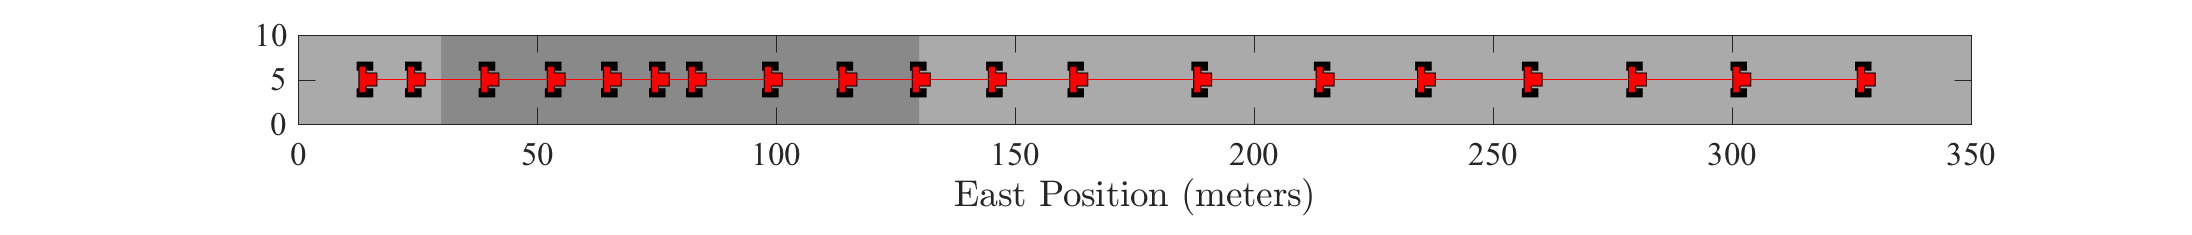
\includegraphics[width = 6.2in, keepaspectratio]{TC_Fail_WC_Suc_2D1Tractor}
    \caption{Two dimensional plot of the red tractors position taken at snapshots in time. The terrain conditions for this tractor are identical to those in Ch. \ref{ch:TCM} and can be referenced in in Table \ref{table:soft_terrain_5tractors_TC} and Fig. \ref{fig:Net_Traction_With_Payload_TC_Both}. The starting and ending terrains are firm and provide plenty of traction while the middle terrain is softer and has a risk of immobilization.}
    \label{fig:TC_Fail_WC_Suc_2D1Tractor}
\end{figure}
\begin{figure}[htbp]
    \centering
    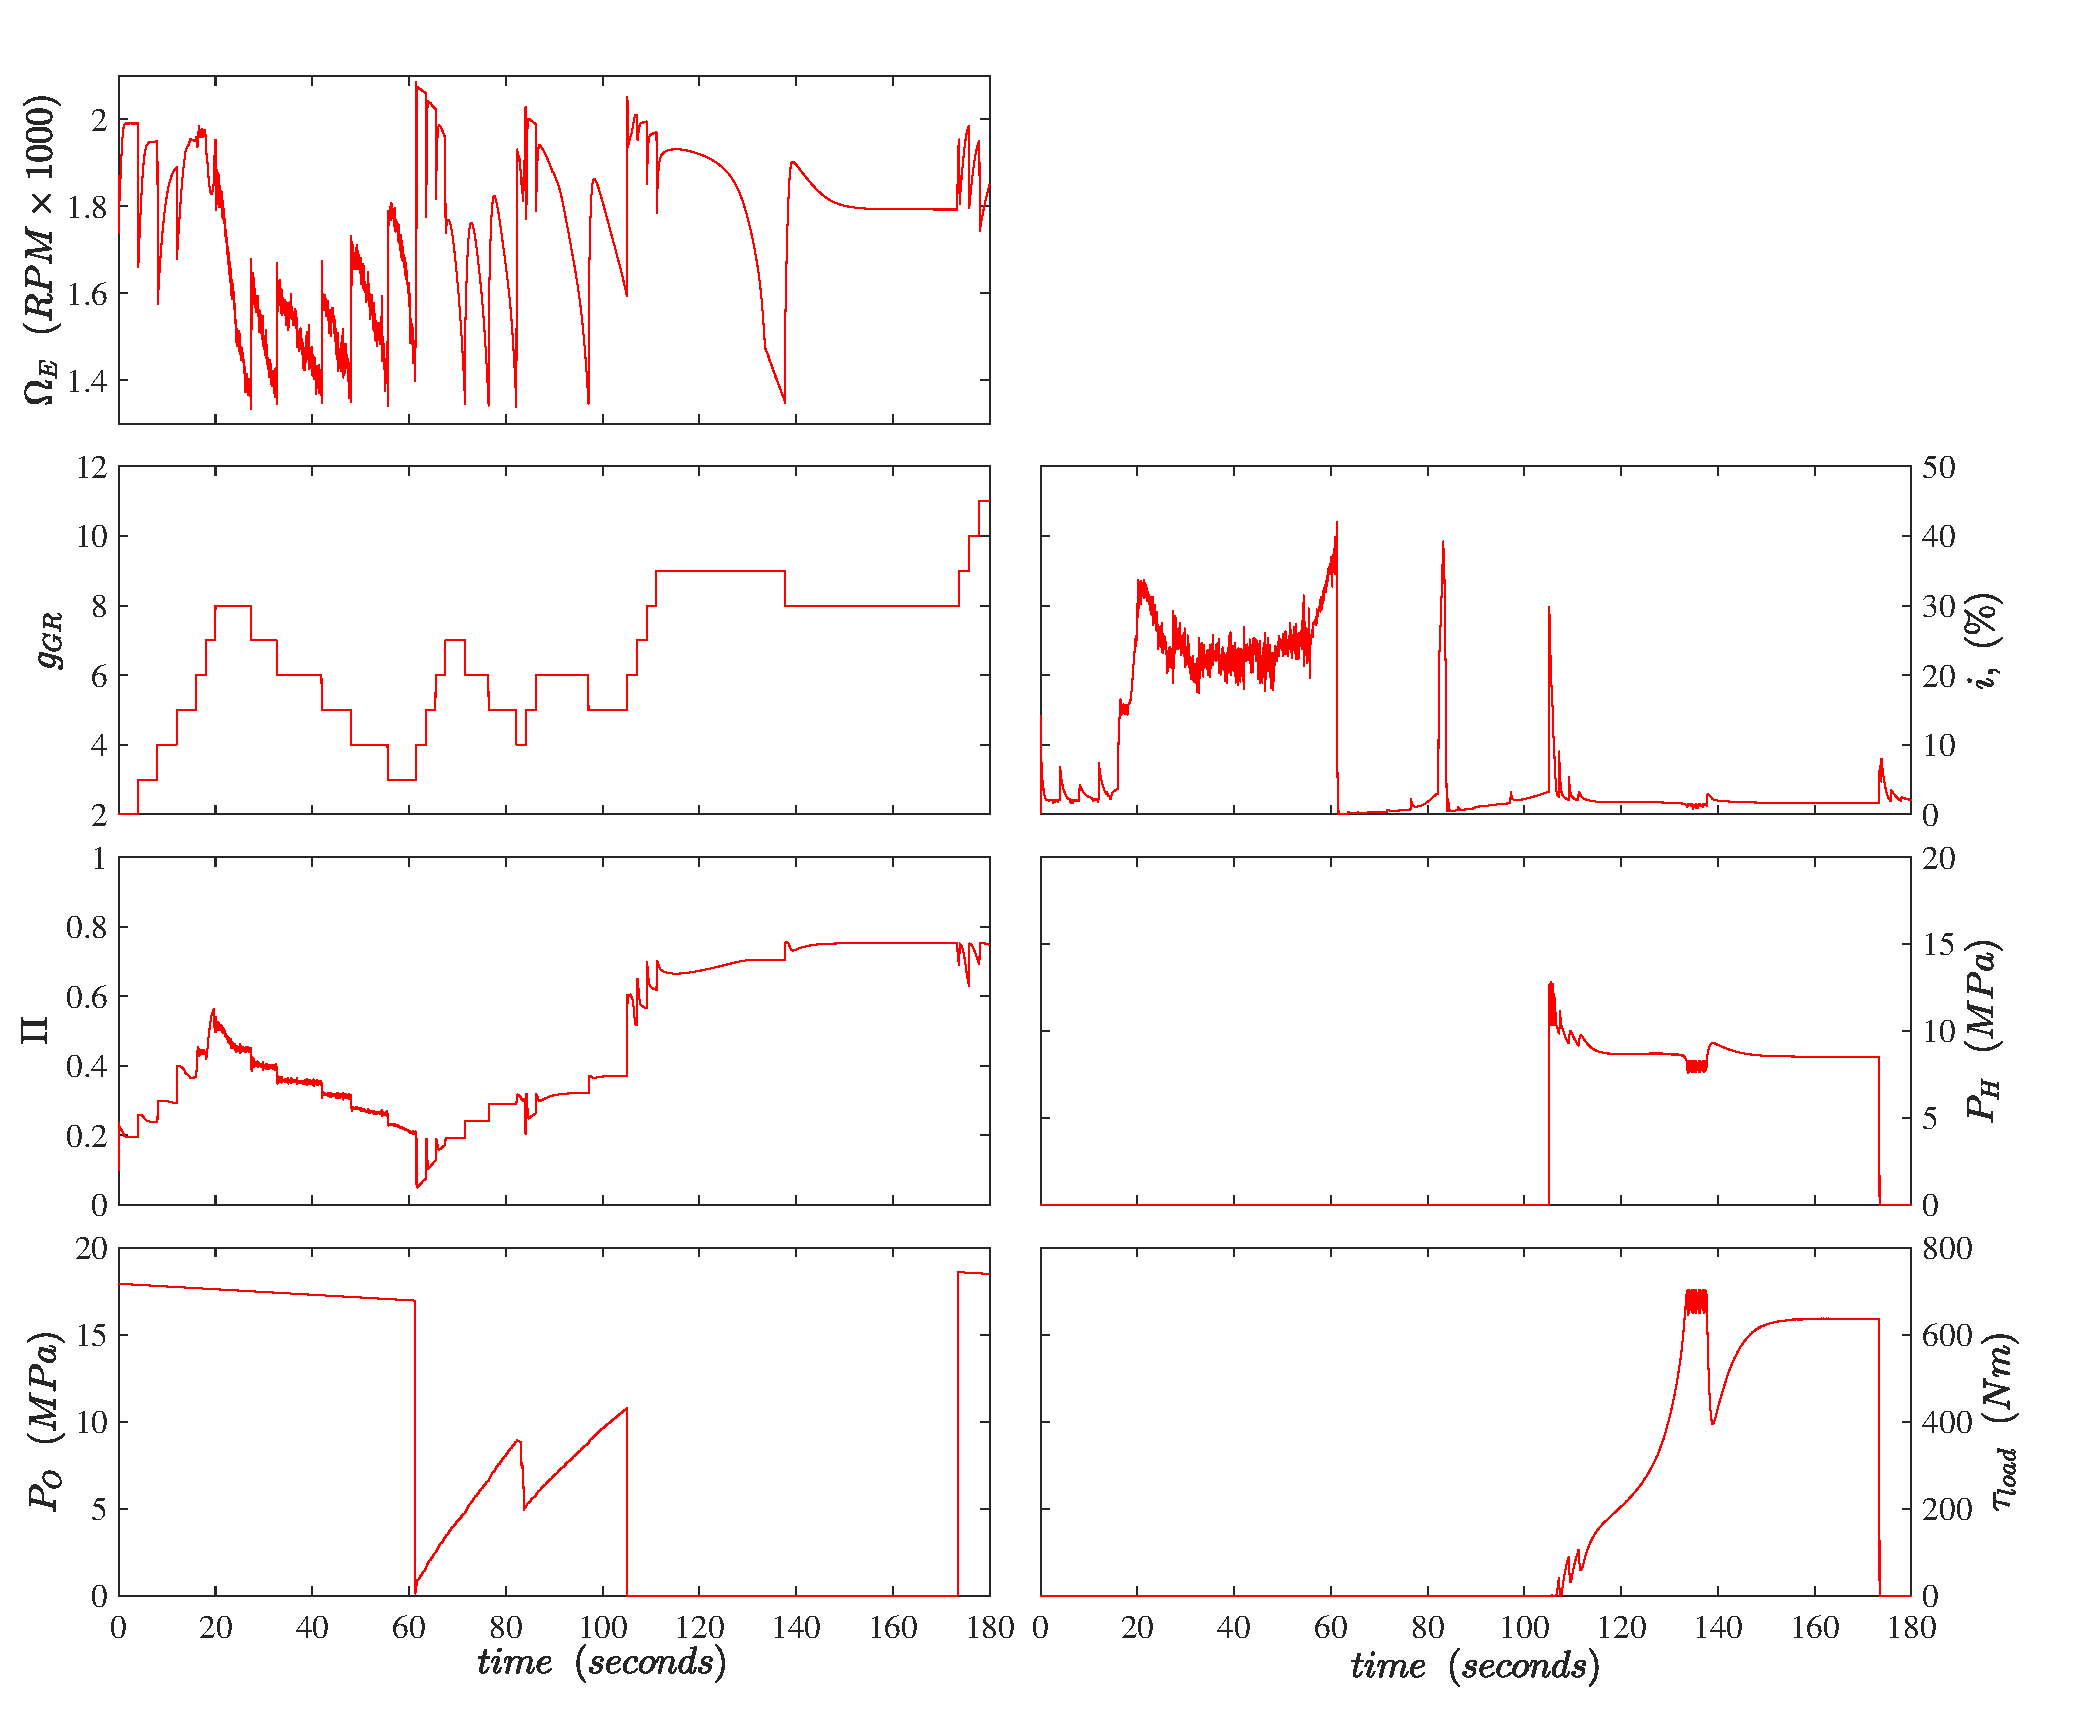
\includegraphics[width = 6in, keepaspectratio]{TC_Fail_WC_Suc_Traj1}
    \caption{Plots of inputs and state variables for red tractor using both the traction control mode and winch control mode. These include throttle and gear selection inputs $\Pi$ and $g_{GR}$ and state variables of engine speed $\Omega_E$, slip $i$, pressure of the H and O nodes in the winch hydraulics $P_H$ and $P_O$ and the load placed on the engine from the winch hydralics $\tau_{load}$.}
    \label{fig:TC_Fail_WC_Suc_Traj1}
\end{figure}
\begin{figure}[htb]
    \centering
    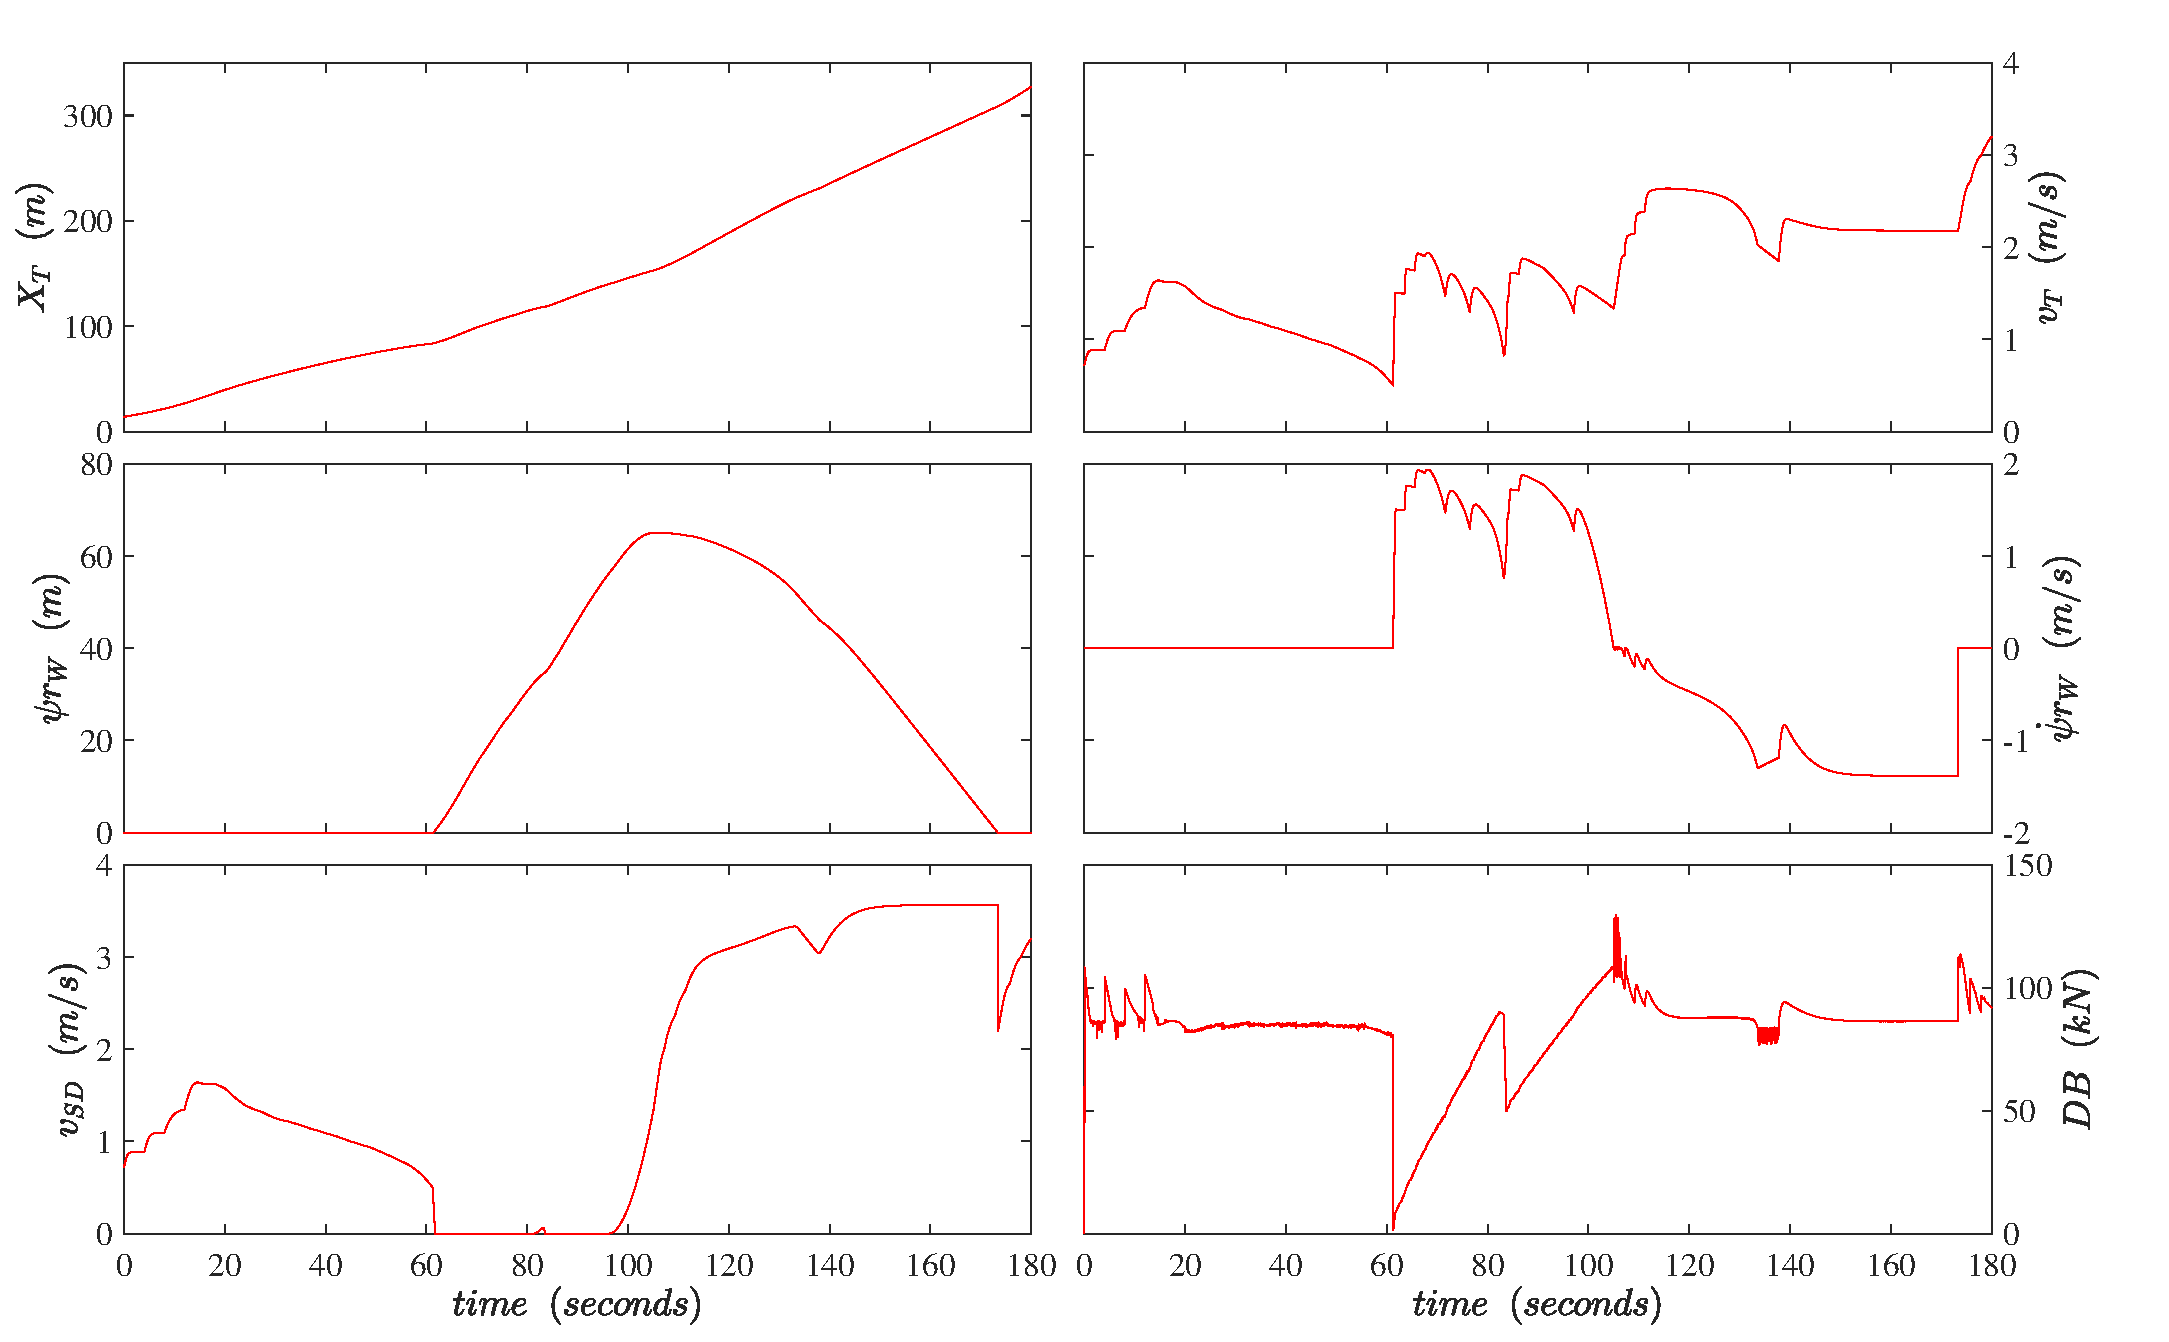
\includegraphics[width = 6in, keepaspectratio]{TC_Fail_WC_Suc_Traj2}
    \caption{Plots of state variables for red tractor using both the traction control mode and winch control mode. These include the tractors east position $X_T$, tractor speed $v_T$, cable length released $\psi r_W$, the speed of cable length be released or being pulled in $\dot{\psi} r_W$, sled speed $v_{SD}$ and drawbar load $DB$.}
    \label{fig:TC_Fail_WC_Suc_Traj2}
\end{figure}
Here, the tractor operates as before until $\sim$60 seconds into the simulation when the winch control mode becomes activated in stage 1.  This can be seen by looking at Fig.'s \ref{fig:TC_Fail_WC_Suc_Traj1} and \ref{fig:TC_Fail_WC_Suc_Traj2} where the slip $i$, pressure in the hydraulics $P_O$, and drawbar load $DB$ all drop to values close to zero to let the payload out. Subsequently, stage 2 is entered and $P_{set}$ is slowly incremented as outlined in algorithm \ref{alg:WIPC}. This can be seen in the slow increase in $P_O$ and in the drawbar load $DB$. At $\sim$83 seconds, the tractor has detected that the drawbar is overloaded and decreases the $P_{set}$ and $incPSI$ values in lines 10 and 11 of algorithm \ref{alg:WIPC}. This rapidly decreases the load on the tractor and increases the drawbar load more slowly for another attempt to initialize the payload recovery. At $\sim$90 seconds of simulation the tractor exits the soft terrain stretch and is able to bring the winch to a locked state where no more cable length is being let out. This can be seen in Fig. \ref{fig:TC_Fail_WC_Suc_Traj2} where $\psi r_W$ is the amount of cable length let out and $\dot{\psi} r_W$ is the speed at which cable is being let out in meters. This process takes $\sim$15 seconds and stage 3 is entered $\sim$105 second into the simulation. The initial kickback from switching the discrete 4 way, 2 position valve puts the I position creates a spike in the hydraulic pressure $P_H$ which highlights the reason for initializing the $P_{set}$ value to a small value of $15\hspace{1mm}psi$ upon transition into stage 3. The $P_{set}$ value is then slowly increased as outlined in algorithm \ref{alg:WIFR} to slowly increase the load on the engine $\tau_{load}$ and the speed at which the payload is pulled in $\dot{\psi} r_W$.

The second of set simulation results will show the effectiveness of the winch control mode's architecture by simulating 4 tractors traversing terrain with no positive $F_{net,DB}$ values for any domain of slip ratios $i$. In addition, the terrain on which the payload must be recovered will not provide a surplus of traction as with the first set of results. 

Figure \ref{fig:WC_4Tractor_2DPlot} shows a two dimensional plot of all tractor positions at snap shots in time. Each tractor is traversing soft terrain patches of varying length in the middle terrain sections. The cyan, green, blue, and red tractors traverse soft terrain lengths of $42\hspace{1mm}m$, $50\hspace{1mm}m$, $60\hspace{1mm}m$, and $30\hspace{1mm}m$ respectively with specific starting and end locations provided in Table \ref{table:middle_terrain_4tractors_WC}. The slip force curves of $i$ versus $F_{net,DB}$ are shown for all soft, middle terrain lengths in the left plot of Fig. \ref{fig:WC_Terrain_Mid_End}. It can be seen that all values are negative across the entire $i$ domain and so the tractors must use their winches to maintain mobility. Terrain parameters for each curve are provided in Table \ref{table:middle_terrain_4tractors_WC}. The end terrain slip-force $i$, $F_{net,DB}$ curves are shown in the right plot of Fig. \ref{table:end_terrain_4tractors_WC}. These terrains provide slightly more traction than those of the soft terrain patches from the simulation results in Ch. \ref{ch:TCM} since the drawbar requirements will be greater for payload recovery. These are more challenging terrains for payload recovery than what was in the first set of simulation results in this section. Trajectories for each tractor are included in Fig.'s \ref{fig:WC_CyanTractor_Traj1}-\ref{fig:WC_RedTractor_Traj2}.
\begin{figure}[hb]
    \centering
    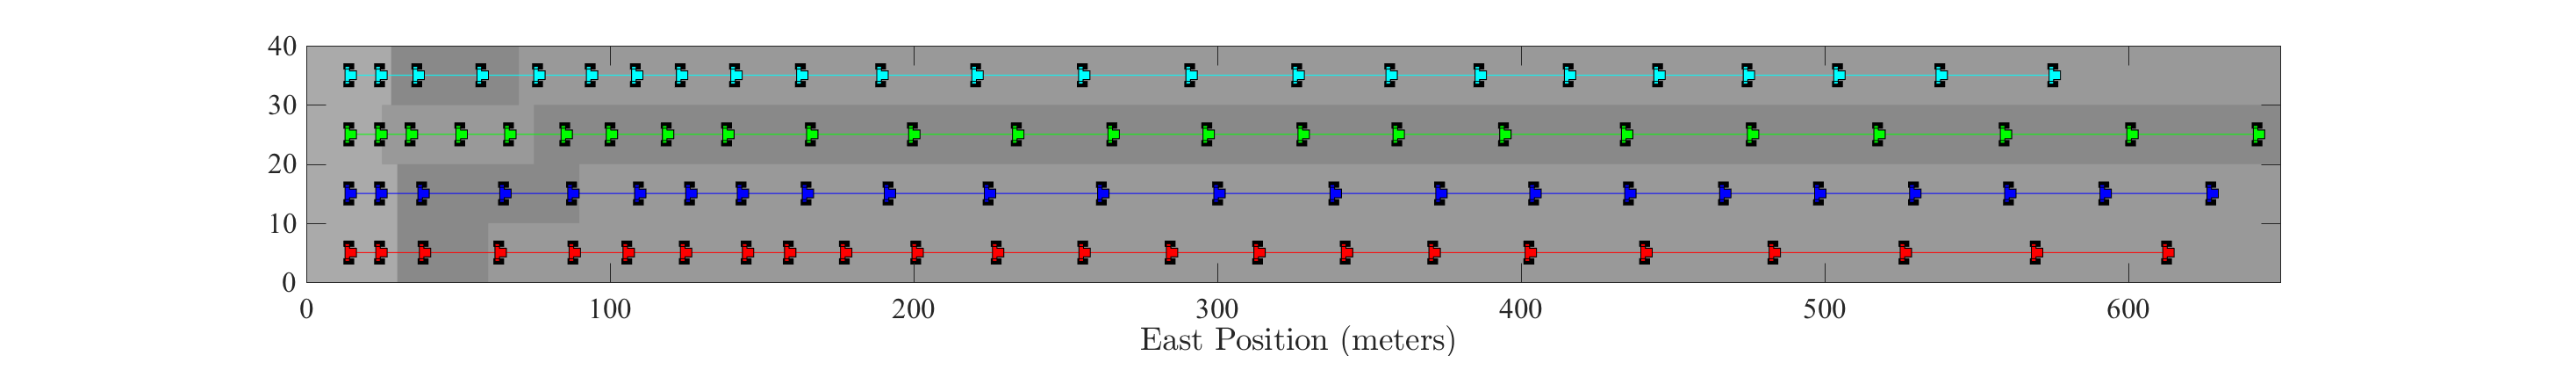
\includegraphics[width = 6 in, keepaspectratio]{WC_4Tractor_2DPlot}
    \caption{Two dimensional plot of four tractors' positions cyan, green, blue and red taken at snapshots in time traversing soft terrain using the winch control mode to maintain mobility. Slip-force curves for relevant terrain are shown Fig. \ref{fig:WC_Terrain_Mid_End} with specifics of terrain parameters and spatial locations in Tables \ref{table:middle_terrain_4tractors_WC}, \ref{table:end_terrain_4tractors_WC} and \ref{table:loc_terrain_4tractors_WC}.}
    \label{fig:WC_4Tractor_2DPlot}
\end{figure}
\begin{figure}[htbp]
    \centering
    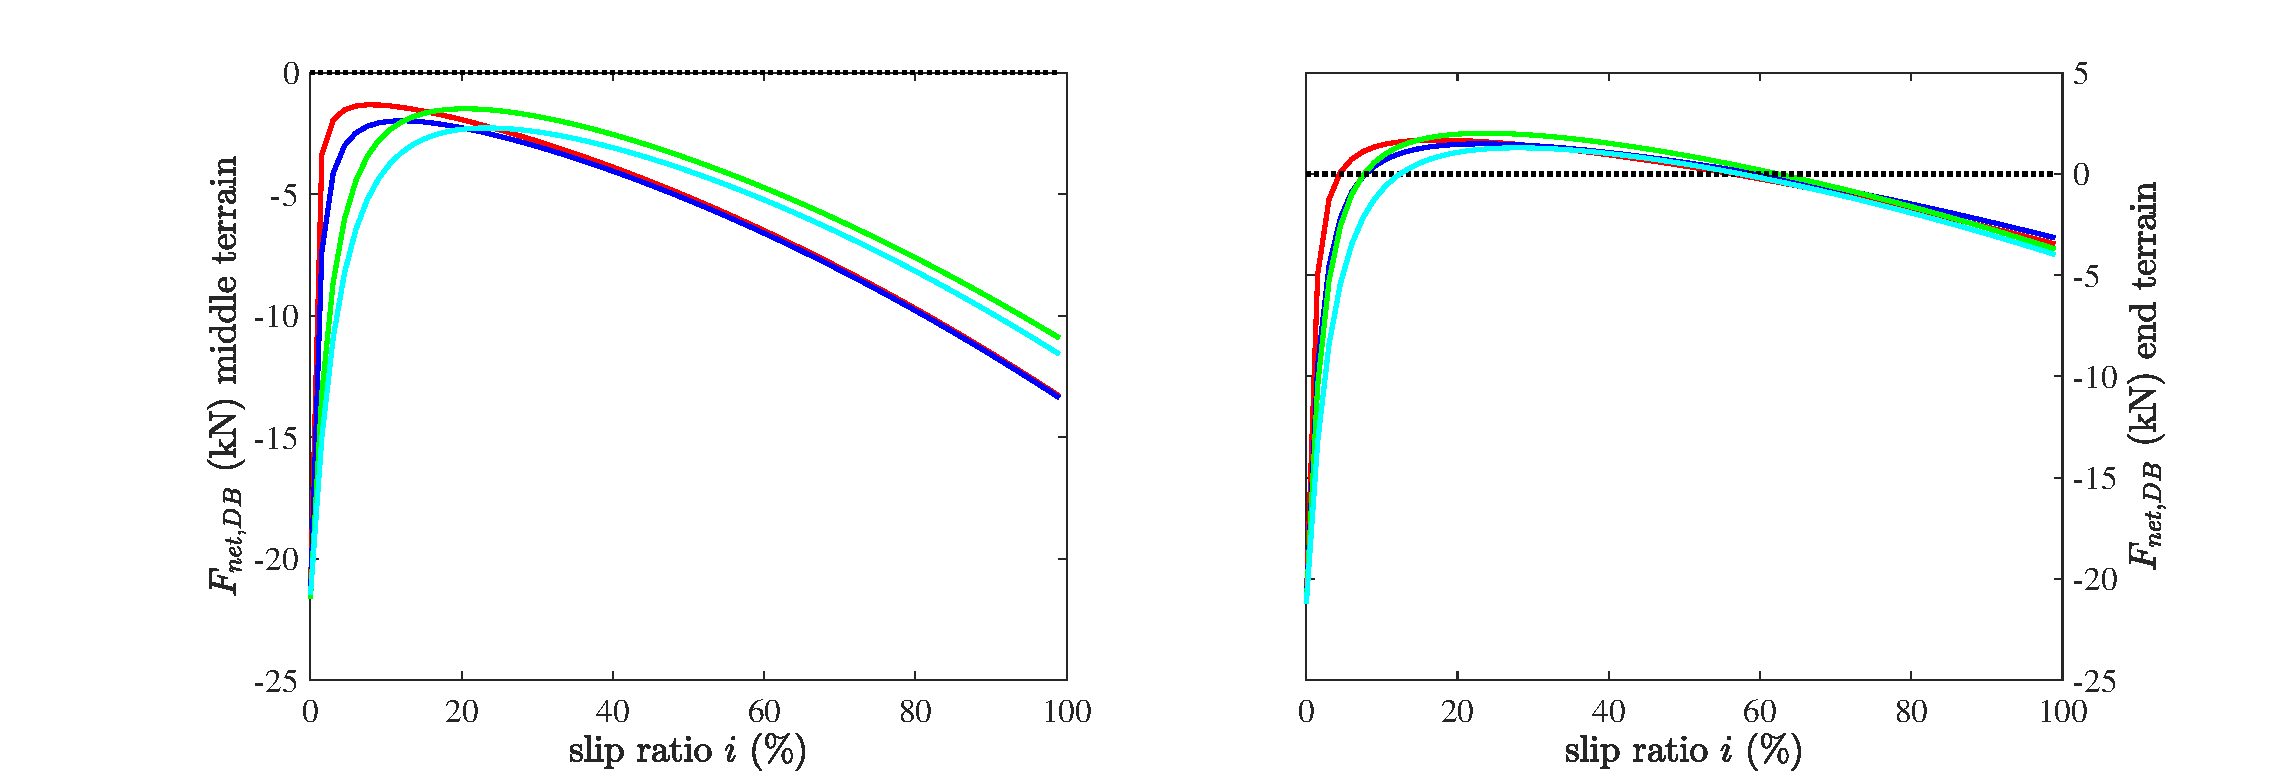
\includegraphics[width = 6in, keepaspectratio]{WC_Terrain_Mid_End}
    \caption{Net traction curves accounting drawbar loading $F_{net,DB}$ for each tractor's middle (left plot) and end (right plot) operating terrain in Fig. \ref{fig:WC_4Tractor_2DPlot}. Curve colors correspond to tractor colors.}
    \label{fig:WC_Terrain_Mid_End}
\end{figure}
\begin{table}[htbp]
\caption{Terrain parameters for middle terrain patch for each of the four tractors}
\label{table:middle_terrain_4tractors_WC}
\begin{center}
\vspace{-5mm}
\begin{tabular}{ |c|c|c|c|c|c|c| } 
 \hline
 tractor color & $c$ & $\Phi$ & $n$ & $k_{eq}$ & $K$ & $S$ \\ 
 \hline
  \vspace{-0.6mm} & \vspace{-0.6mm} & \vspace{-0.6mm} & \vspace{-0.6mm} & \vspace{-0.6mm} & \vspace{-0.6mm} & \vspace{-0.6mm}  \\ 
 \hline
 cyan & $3\hspace{1mm}kPa$ & $17.8^o$ & $1$ & $375\hspace{1mm}(kN/m^{n+2})$ & $6.8\hspace{1mm}cm$ & $ 90\%/33\%$ \\ 
 \hline
 green & $3\hspace{1mm}kPa$ & $18.15^o$ & $1$ & $320\hspace{1mm}(kN/m^{n+2})$ & $4.9\hspace{1mm}cm$ & $80\%/33\%$ \\ 
 \hline
 blue & $2\hspace{1mm}kPa$ & $17.8^o$ & $1$ & $300\hspace{1mm}(kN/m^{n+2})$ & $1.7\hspace{1mm}cm$ & $80\%/33\%$ \\ 
 \hline
 red & $2\hspace{1mm}kPa$ & $17.8^o$ & $1$ & $300\hspace{1mm}(kN/m^{n+2})$ & $0.7\hspace{1mm}cm$ & $80\%/33\%$ \\ 
 \hline
\end{tabular}
\end{center}
\end{table}
\begin{table}[htbp]
\caption{Terrain parameters for end terrain patch for each of the four tractors}
\label{table:end_terrain_4tractors_WC}
\begin{center}
\vspace{-5mm}
\begin{tabular}{ |c|c|c|c|c|c|c| } 
 \hline
 tractor color & $c$ & $\Phi$ & $n$ & $k_{eq}$ & $K$ & $S$ \\ 
 \hline
  \vspace{-0.6mm} & \vspace{-0.6mm} & \vspace{-0.6mm} & \vspace{-0.6mm} & \vspace{-0.6mm} & \vspace{-0.6mm} & \vspace{-0.6mm}  \\ 
 \hline
 cyan & $4.7\hspace{1mm}kPa$ & $18^o$ & $1$ & $500\hspace{1mm}(kN/m^{n+2})$ & $6\hspace{1mm}cm$ & $ 90\%/33\%$ \\ 
 \hline
 green & $5.1\hspace{1mm}kPa$ & $17.6^o$ & $1$ & $500\hspace{1mm}(kN/m^{n+2})$ & $4\hspace{1mm}cm$ & $80\%/33\%$ \\ 
 \hline
 blue & $3.3\hspace{1mm}kPa$ & $19^o$ & $1$ & $500\hspace{1mm}(kN/m^{n+2})$ & $3.3\hspace{1mm}cm$ & $70\%/33\%$ \\ 
 \hline
 red & $3\hspace{1mm}kPa$ & $19^o$ & $1$ & $300\hspace{1mm}(kN/m^{n+2})$ & $1.7\hspace{1mm}cm$ & $70\%/33\%$ \\ 
 \hline
\end{tabular}
\end{center}
\end{table}
\begin{table}[htbp]
\caption{Terrain parameters for end terrain patch for each of the four tractors}
\label{table:loc_terrain_4tractors_WC}
\begin{center}
\vspace{-5mm}
\begin{tabular}{ |c|c|c| } 
 \hline
 tractor color & middle terrain start location & middel terrain end location \\ 
 \hline
  \vspace{-1.4mm} & \vspace{-1.4mm} & \vspace{-1.4mm}  \\ 
 \hline
 cyan & $28\hspace{1mm}m$ & $70\hspace{1mm}m$ \\ 
 \hline
 green & $25\hspace{1mm}m$ & $75\hspace{1mm}m$  \\ 
 \hline
 blue & $30\hspace{1mm}m$ & $90\hspace{1mm}m$ \\ 
 \hline
 red & $30\hspace{1mm}m$ & $60\hspace{1mm}m$  \\ 
 \hline
\end{tabular}
\end{center}
\end{table}
The plots in these figures are annotated to highlight transitions between stages in the winch control mode and actions taken in each stage which are outlined in the previous sections of the chapter. The results show that the architecture for the winch control mode is robust to different operating conditions of soft terrain length and the operating terrain on which payloads must be recovered.

The development of this heuristic based approach was made possible by the model development form Ch. \ref{ch:RMBDW} that allows for numerous simulation experiments that all for testing across a variety of conditions. The only limitation with this approach is that the terrain on which the payload is initially attempted to be recovered on must yield a positive value for $F_{net,DB}$ across some domain of slip values for $i \leq 20\%$. Otherwise the payload will not be recovered. To account for this, information or bounds of the terrain properties in which the vehicle operates can be established or the $20\%$ can be used as a default value that tractor operaters may overide.
\begin{figure}[p]
    \centering
    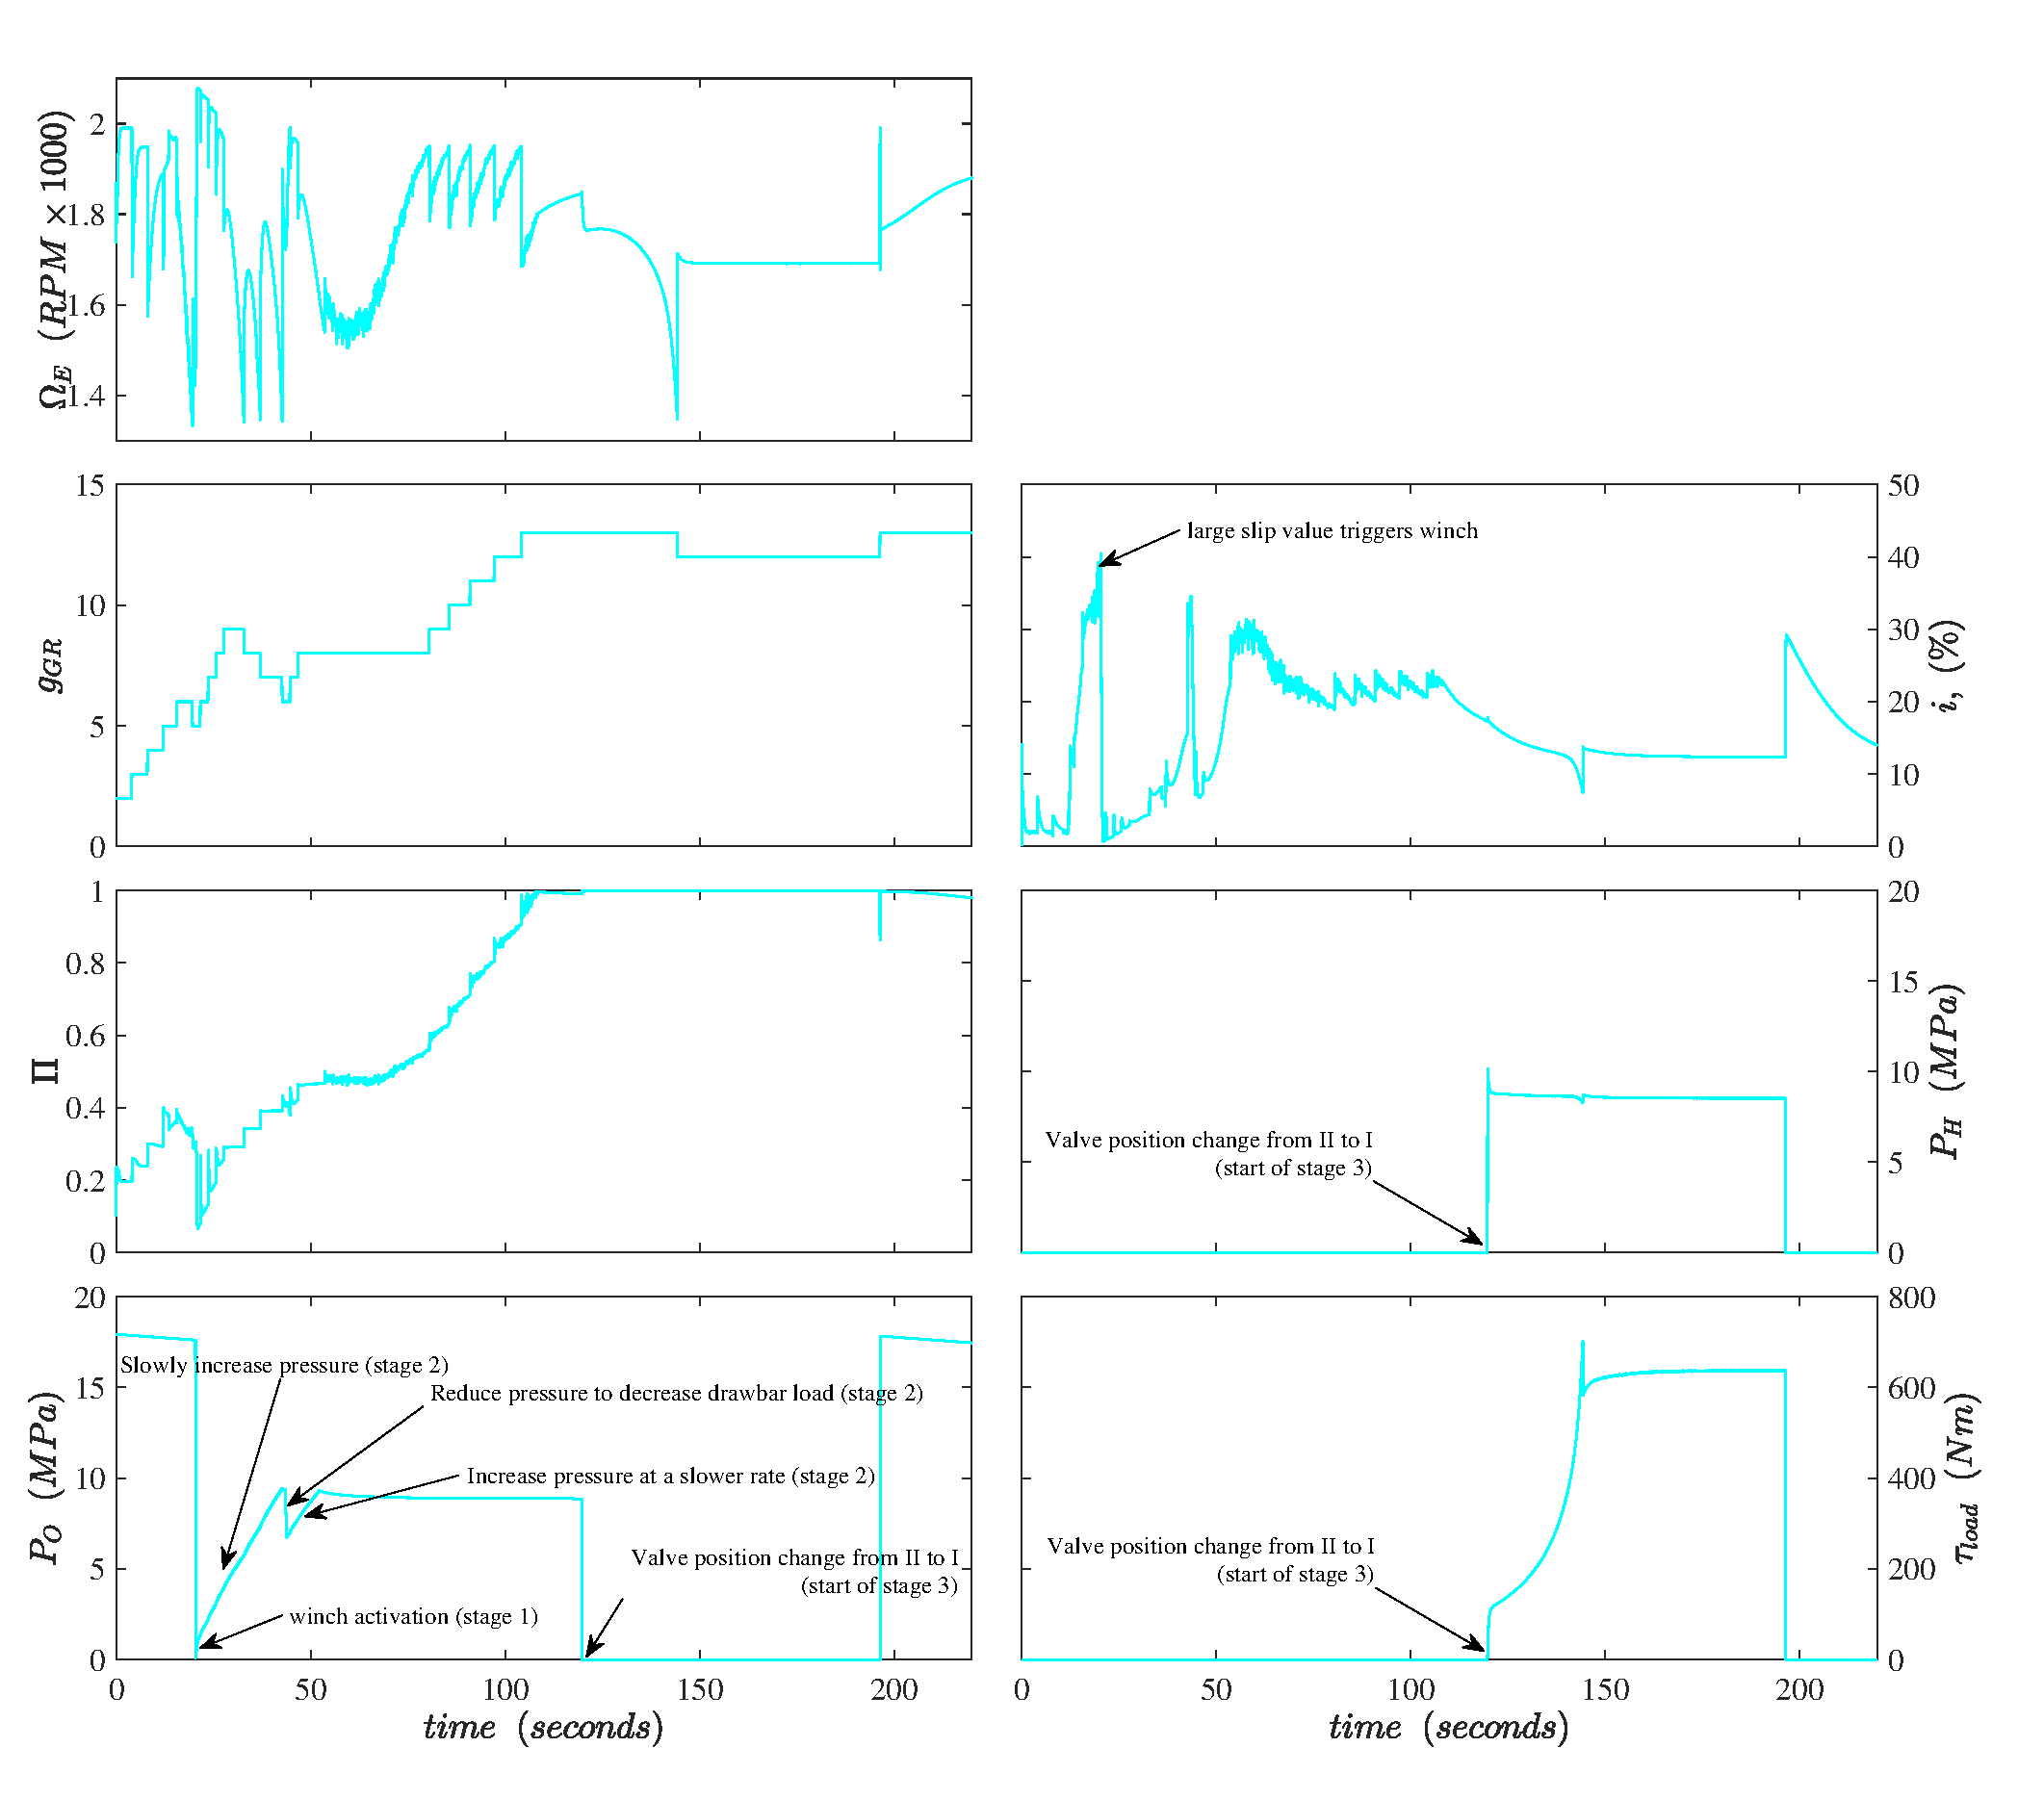
\includegraphics[width = 6in, keepaspectratio]{WC_CyanTractor_Traj1}
    \caption{Plots of inputs and state variables for the cyan tractor using both the traction control mode and winch control mode. These include throttle and gear selection inputs $\Pi$ and $g_{GR}$ and state variables of engine speed $\Omega_E$, slip $i$, pressure of the H and O nodes in the winch hydraulics $P_H$ and $P_O$ and the load placed on the engine from the winch hydralics $\tau_{load}$.}
    \label{fig:WC_CyanTractor_Traj1}
\end{figure}
\begin{figure}[p]
    \centering
    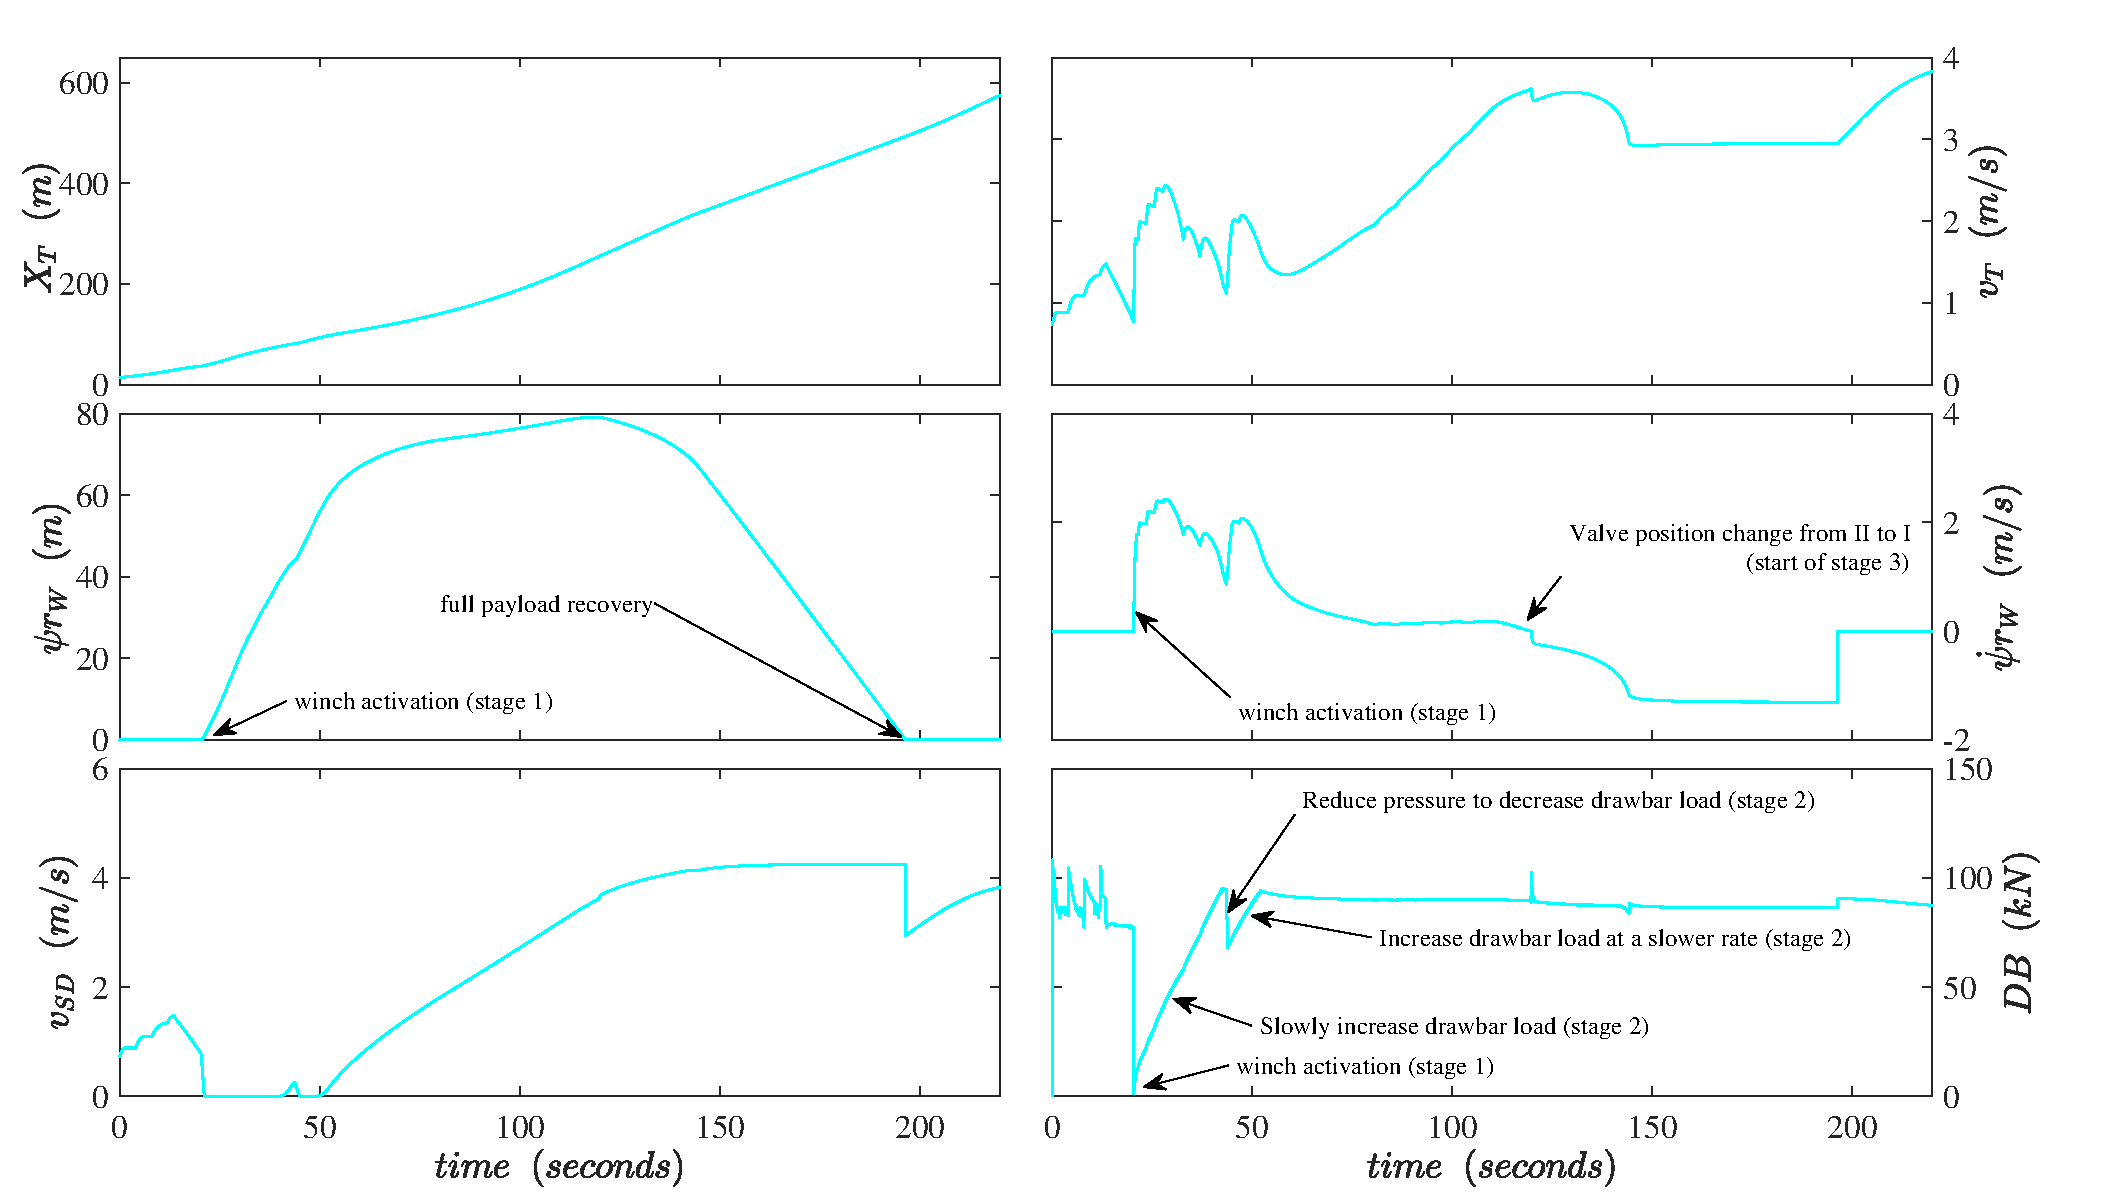
\includegraphics[width = 6in, keepaspectratio]{WC_CyanTractor_Traj2}
    \caption{Plots of state variables for the cyan tractor using both the traction control mode and winch control mode. These include the tractors east position $X_T$, tractor speed $v_T$, cable length released $\psi r_W$, the speed of cable length be released or being pulled in $\dot{\psi} r_W$, sled speed $v_{SD}$ and drawbar load $DB$.}
    \label{fig:WC_CyanTractor_Traj2}
\end{figure}
\begin{figure}[p]
    \centering
    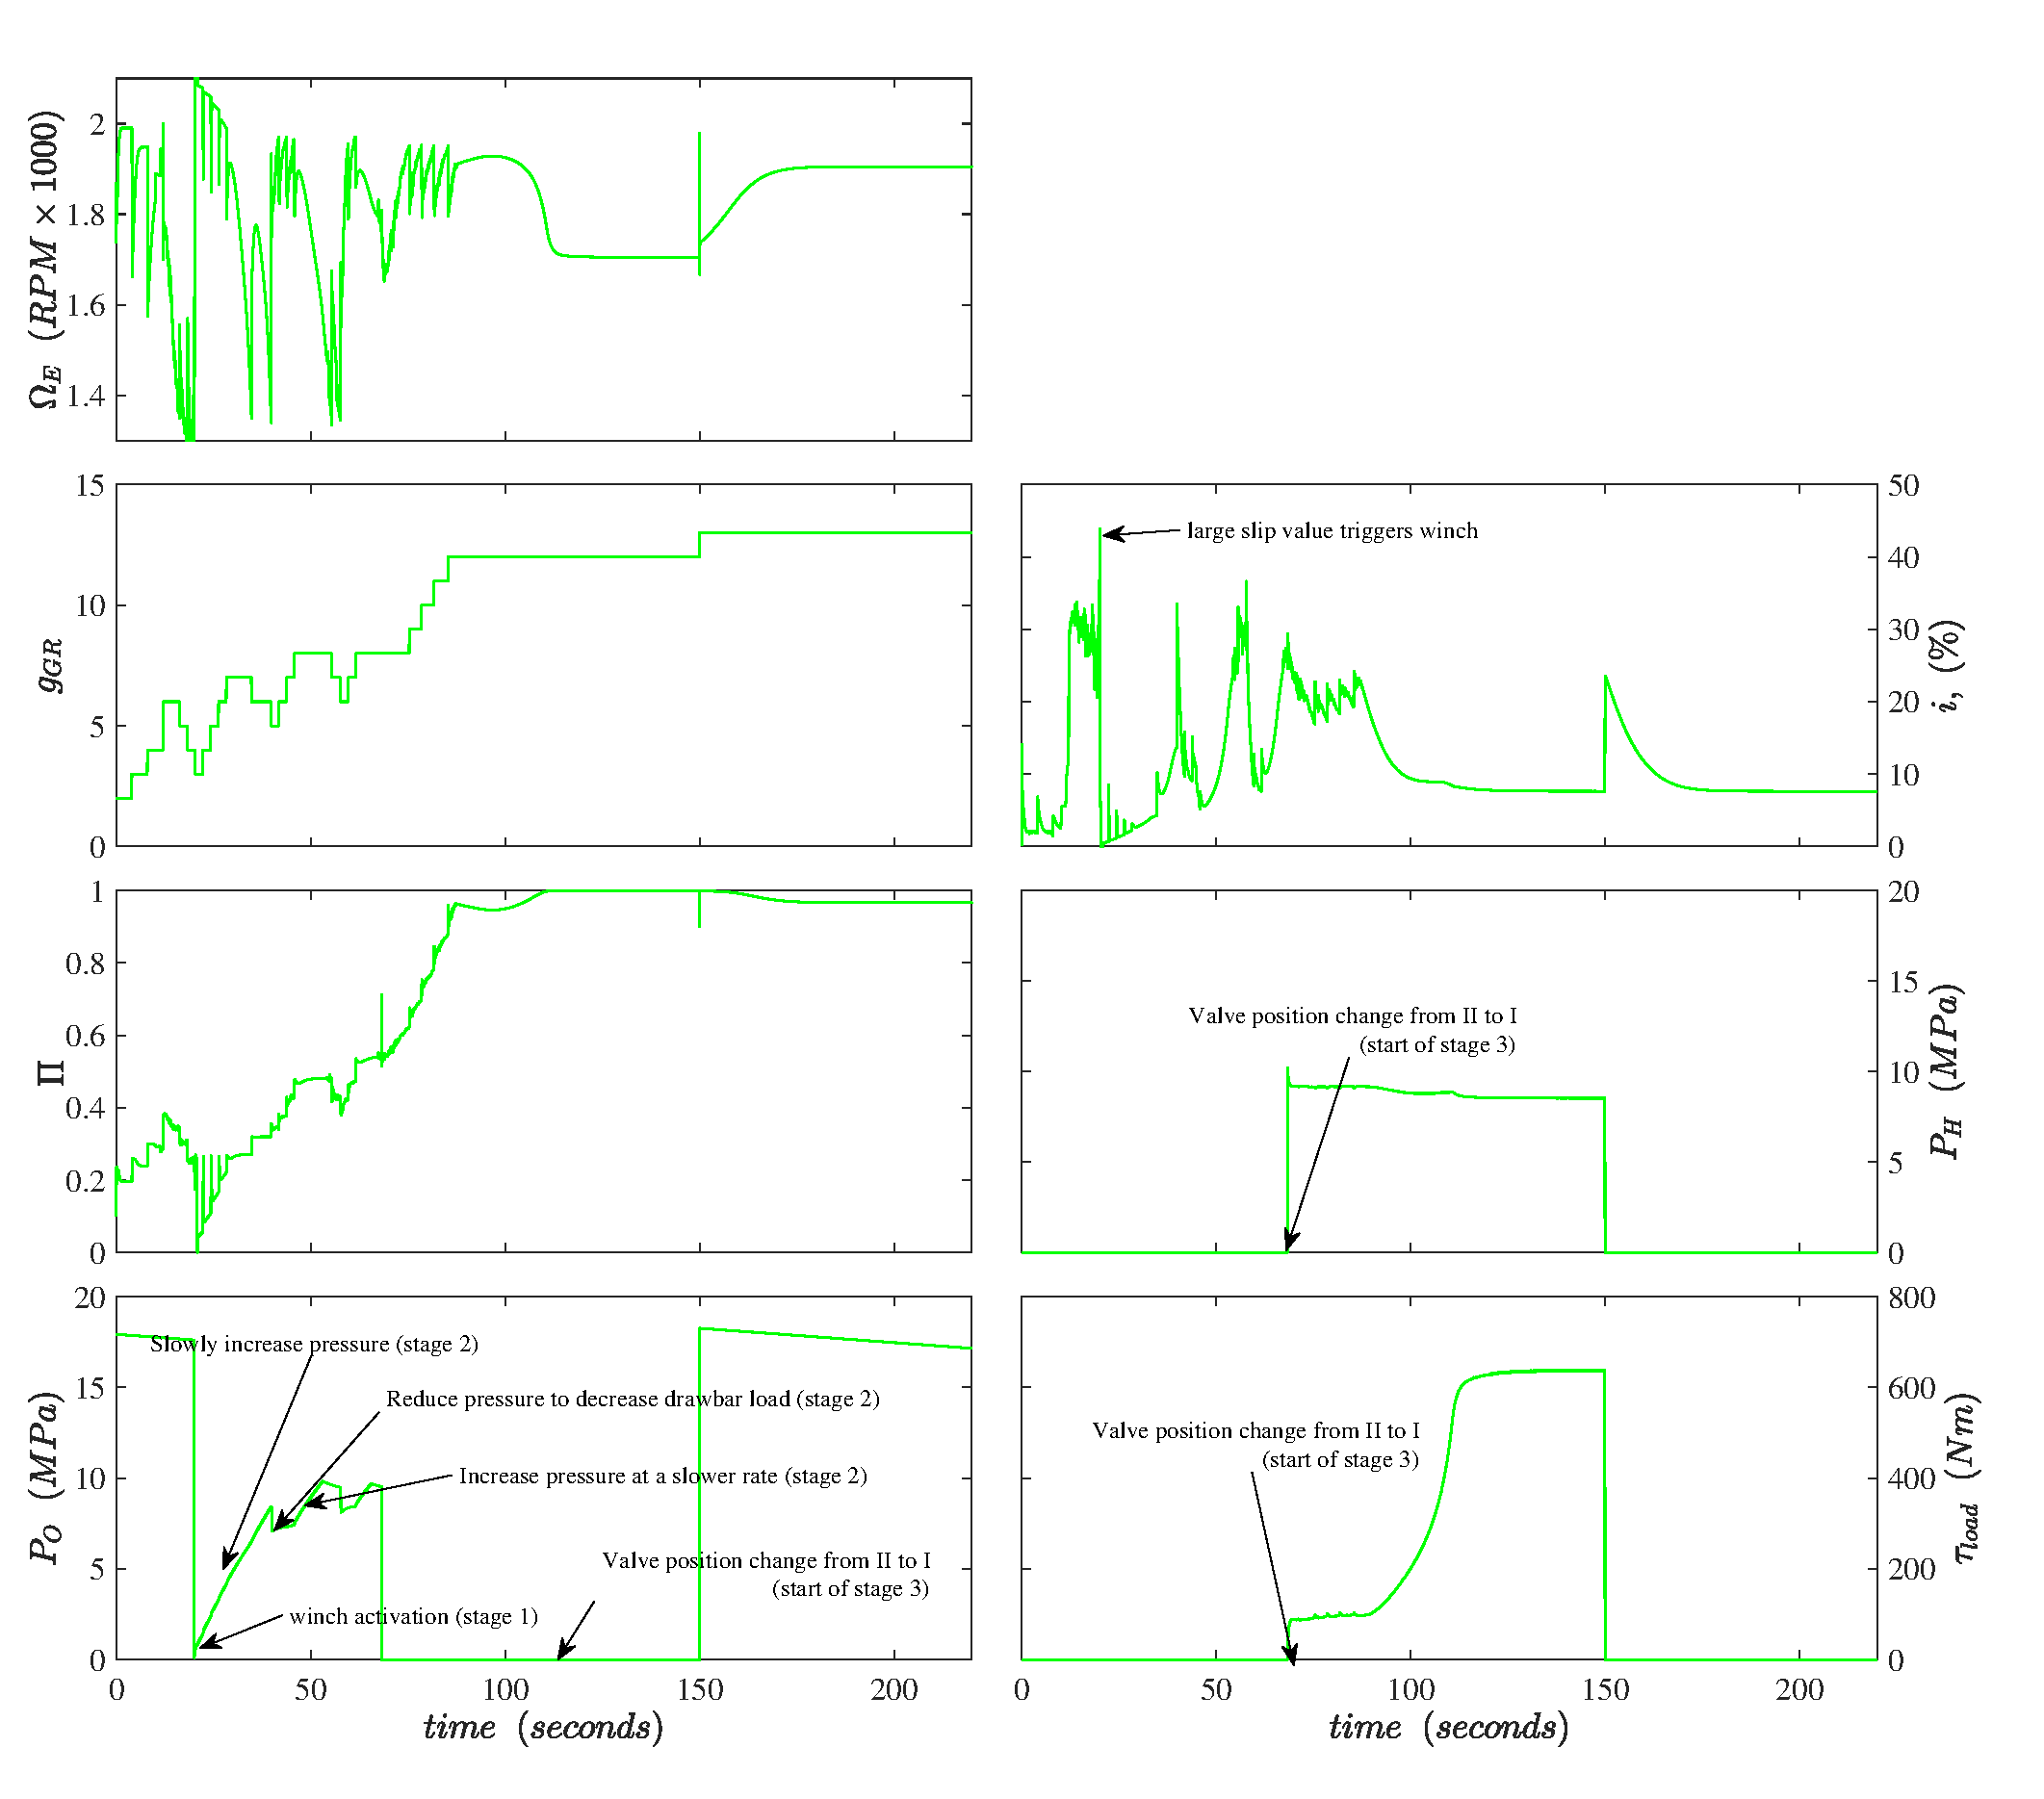
\includegraphics[width = 6in, keepaspectratio]{WC_GreenTractor_Traj1}
    \caption{Plots of inputs and state variables for the green tractor using both the traction control mode and winch control mode. These include throttle and gear selection inputs $\Pi$ and $g_{GR}$ and state variables of engine speed $\Omega_E$, slip $i$, pressure of the H and O nodes in the winch hydraulics $P_H$ and $P_O$ and the load placed on the engine from the winch hydralics $\tau_{load}$.}
    \label{fig:WC_GreenTractor_Traj1}
\end{figure}
\begin{figure}[p]
    \centering
    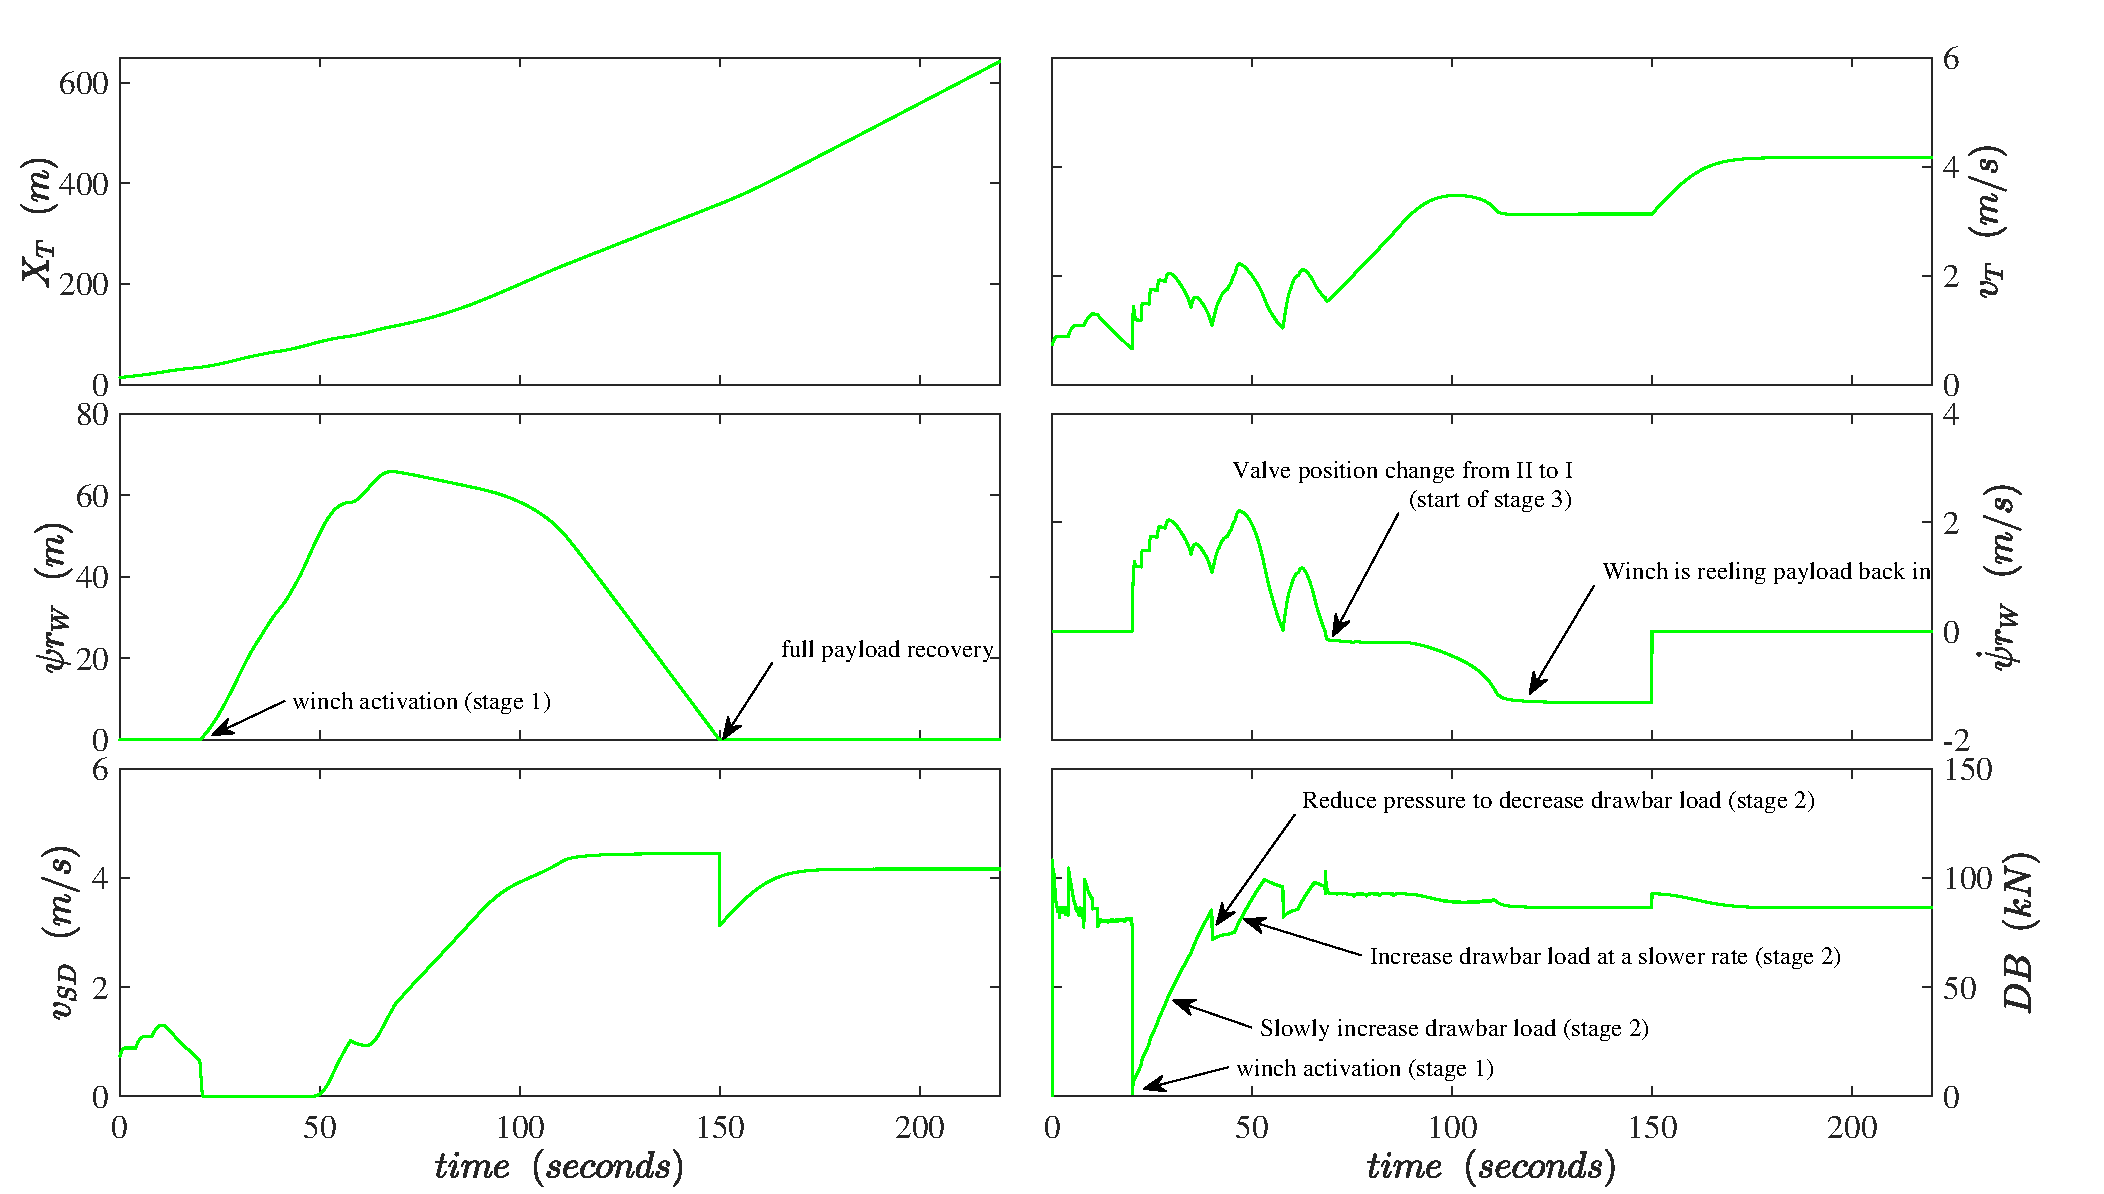
\includegraphics[width = 6in, keepaspectratio]{WC_GreenTractor_Traj2}
    \caption{Plots of state variables for the green tractor using both the traction control mode and winch control mode. These include the tractors east position $X_T$, tractor speed $v_T$, cable length released $\psi r_W$, the speed of cable length be released or being pulled in $\dot{\psi} r_W$, sled speed $v_{SD}$ and drawbar load $DB$.}
    \label{fig:WC_GreenTractor_Traj2}
\end{figure}
\begin{figure}[hp]
    \centering
    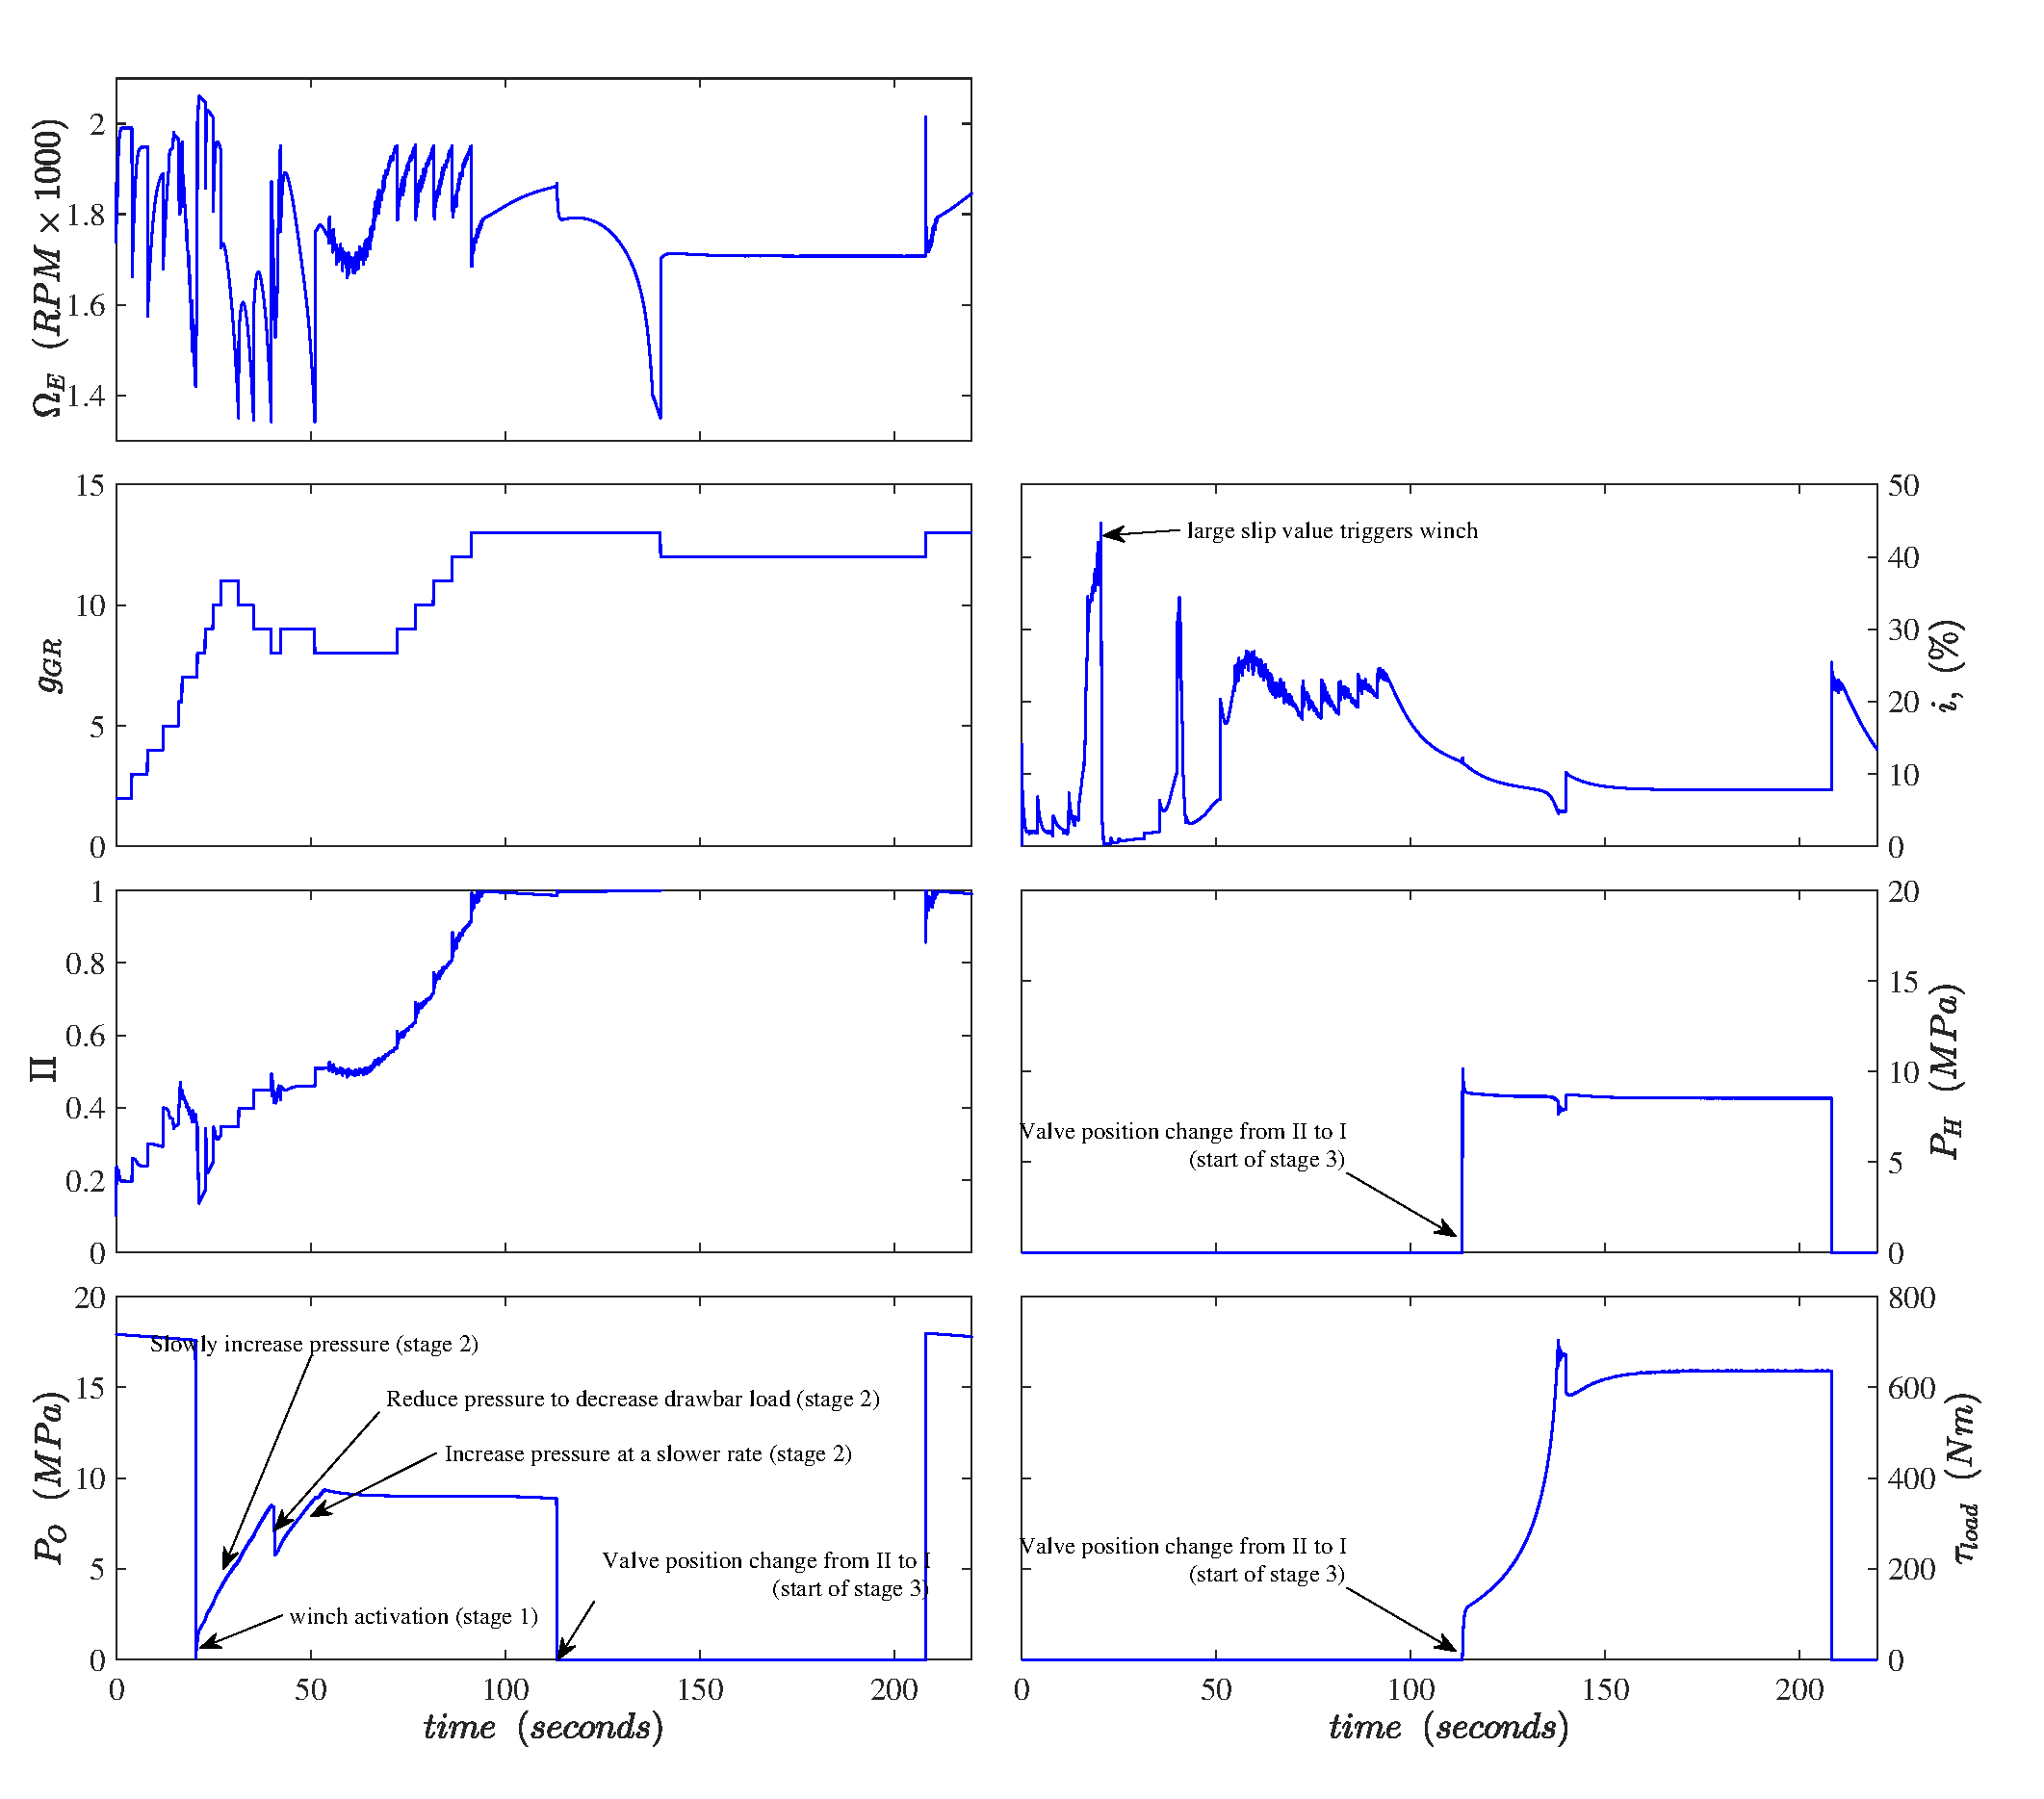
\includegraphics[width = 6in, keepaspectratio]{WC_BlueTractor_Traj1}
    \caption{Plots of inputs and state variables for the blue tractor using both the traction control mode and winch control mode. These include throttle and gear selection inputs $\Pi$ and $g_{GR}$ and state variables of engine speed $\Omega_E$, slip $i$, pressure of the H and O nodes in the winch hydraulics $P_H$ and $P_O$ and the load placed on the engine from the winch hydralics $\tau_{load}$.}
    \label{fig:WC_BlueTractor_Traj1}
\end{figure}
\begin{figure}[p]
    \centering
    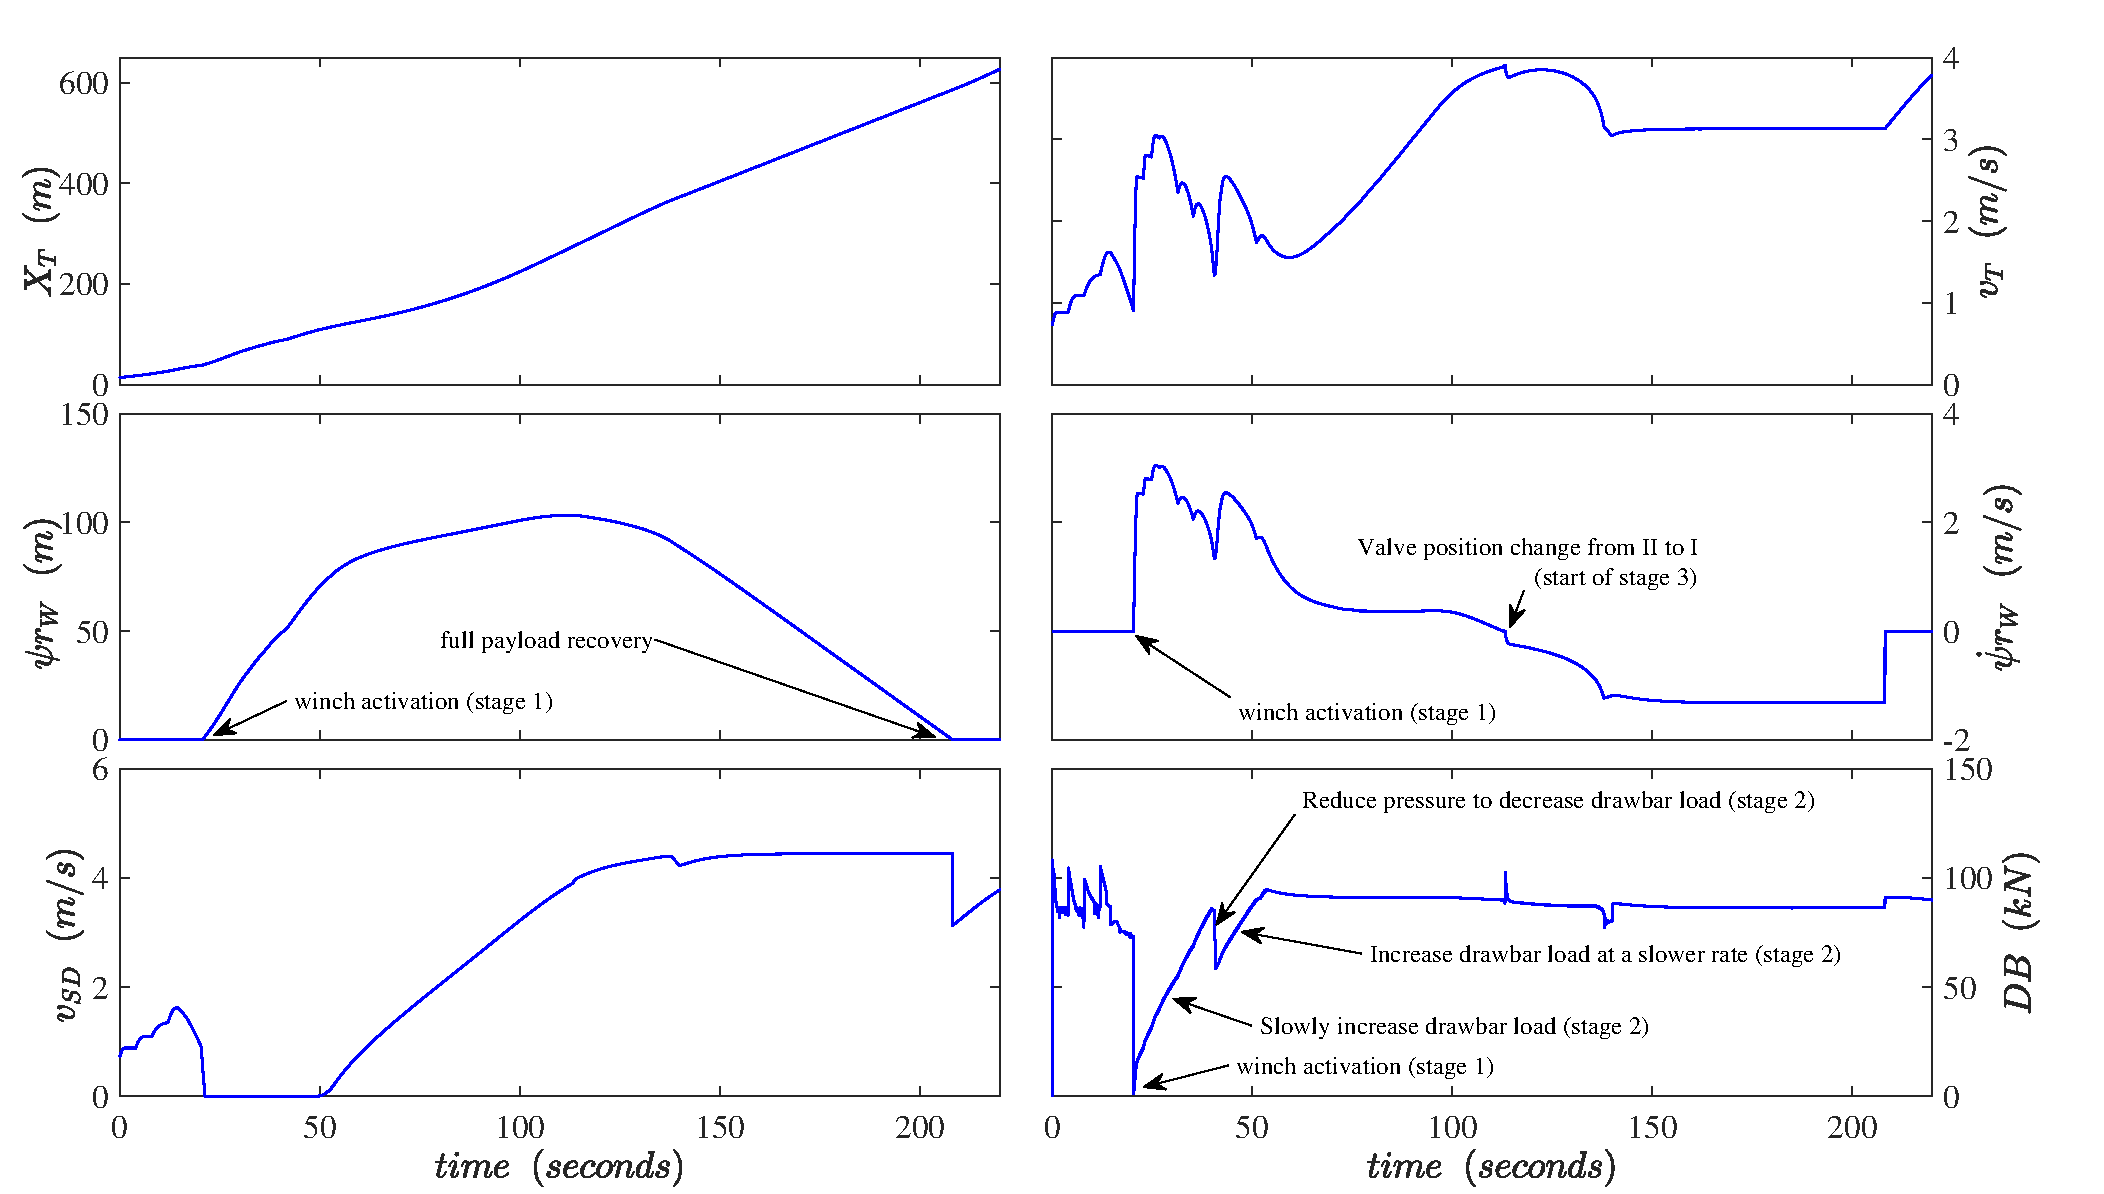
\includegraphics[width = 6in, keepaspectratio]{WC_BlueTractor_Traj2}
    \caption{Plots of state variables for the blue tractor using both the traction control mode and winch control mode. These include the tractors east position $X_T$, tractor speed $v_T$, cable length released $\psi r_W$, the speed of cable length be released or being pulled in $\dot{\psi} r_W$, sled speed $v_{SD}$ and drawbar load $DB$.}
    \label{fig:WC_BlueTractor_Traj2}
\end{figure}
\begin{figure}[p]
    \centering
    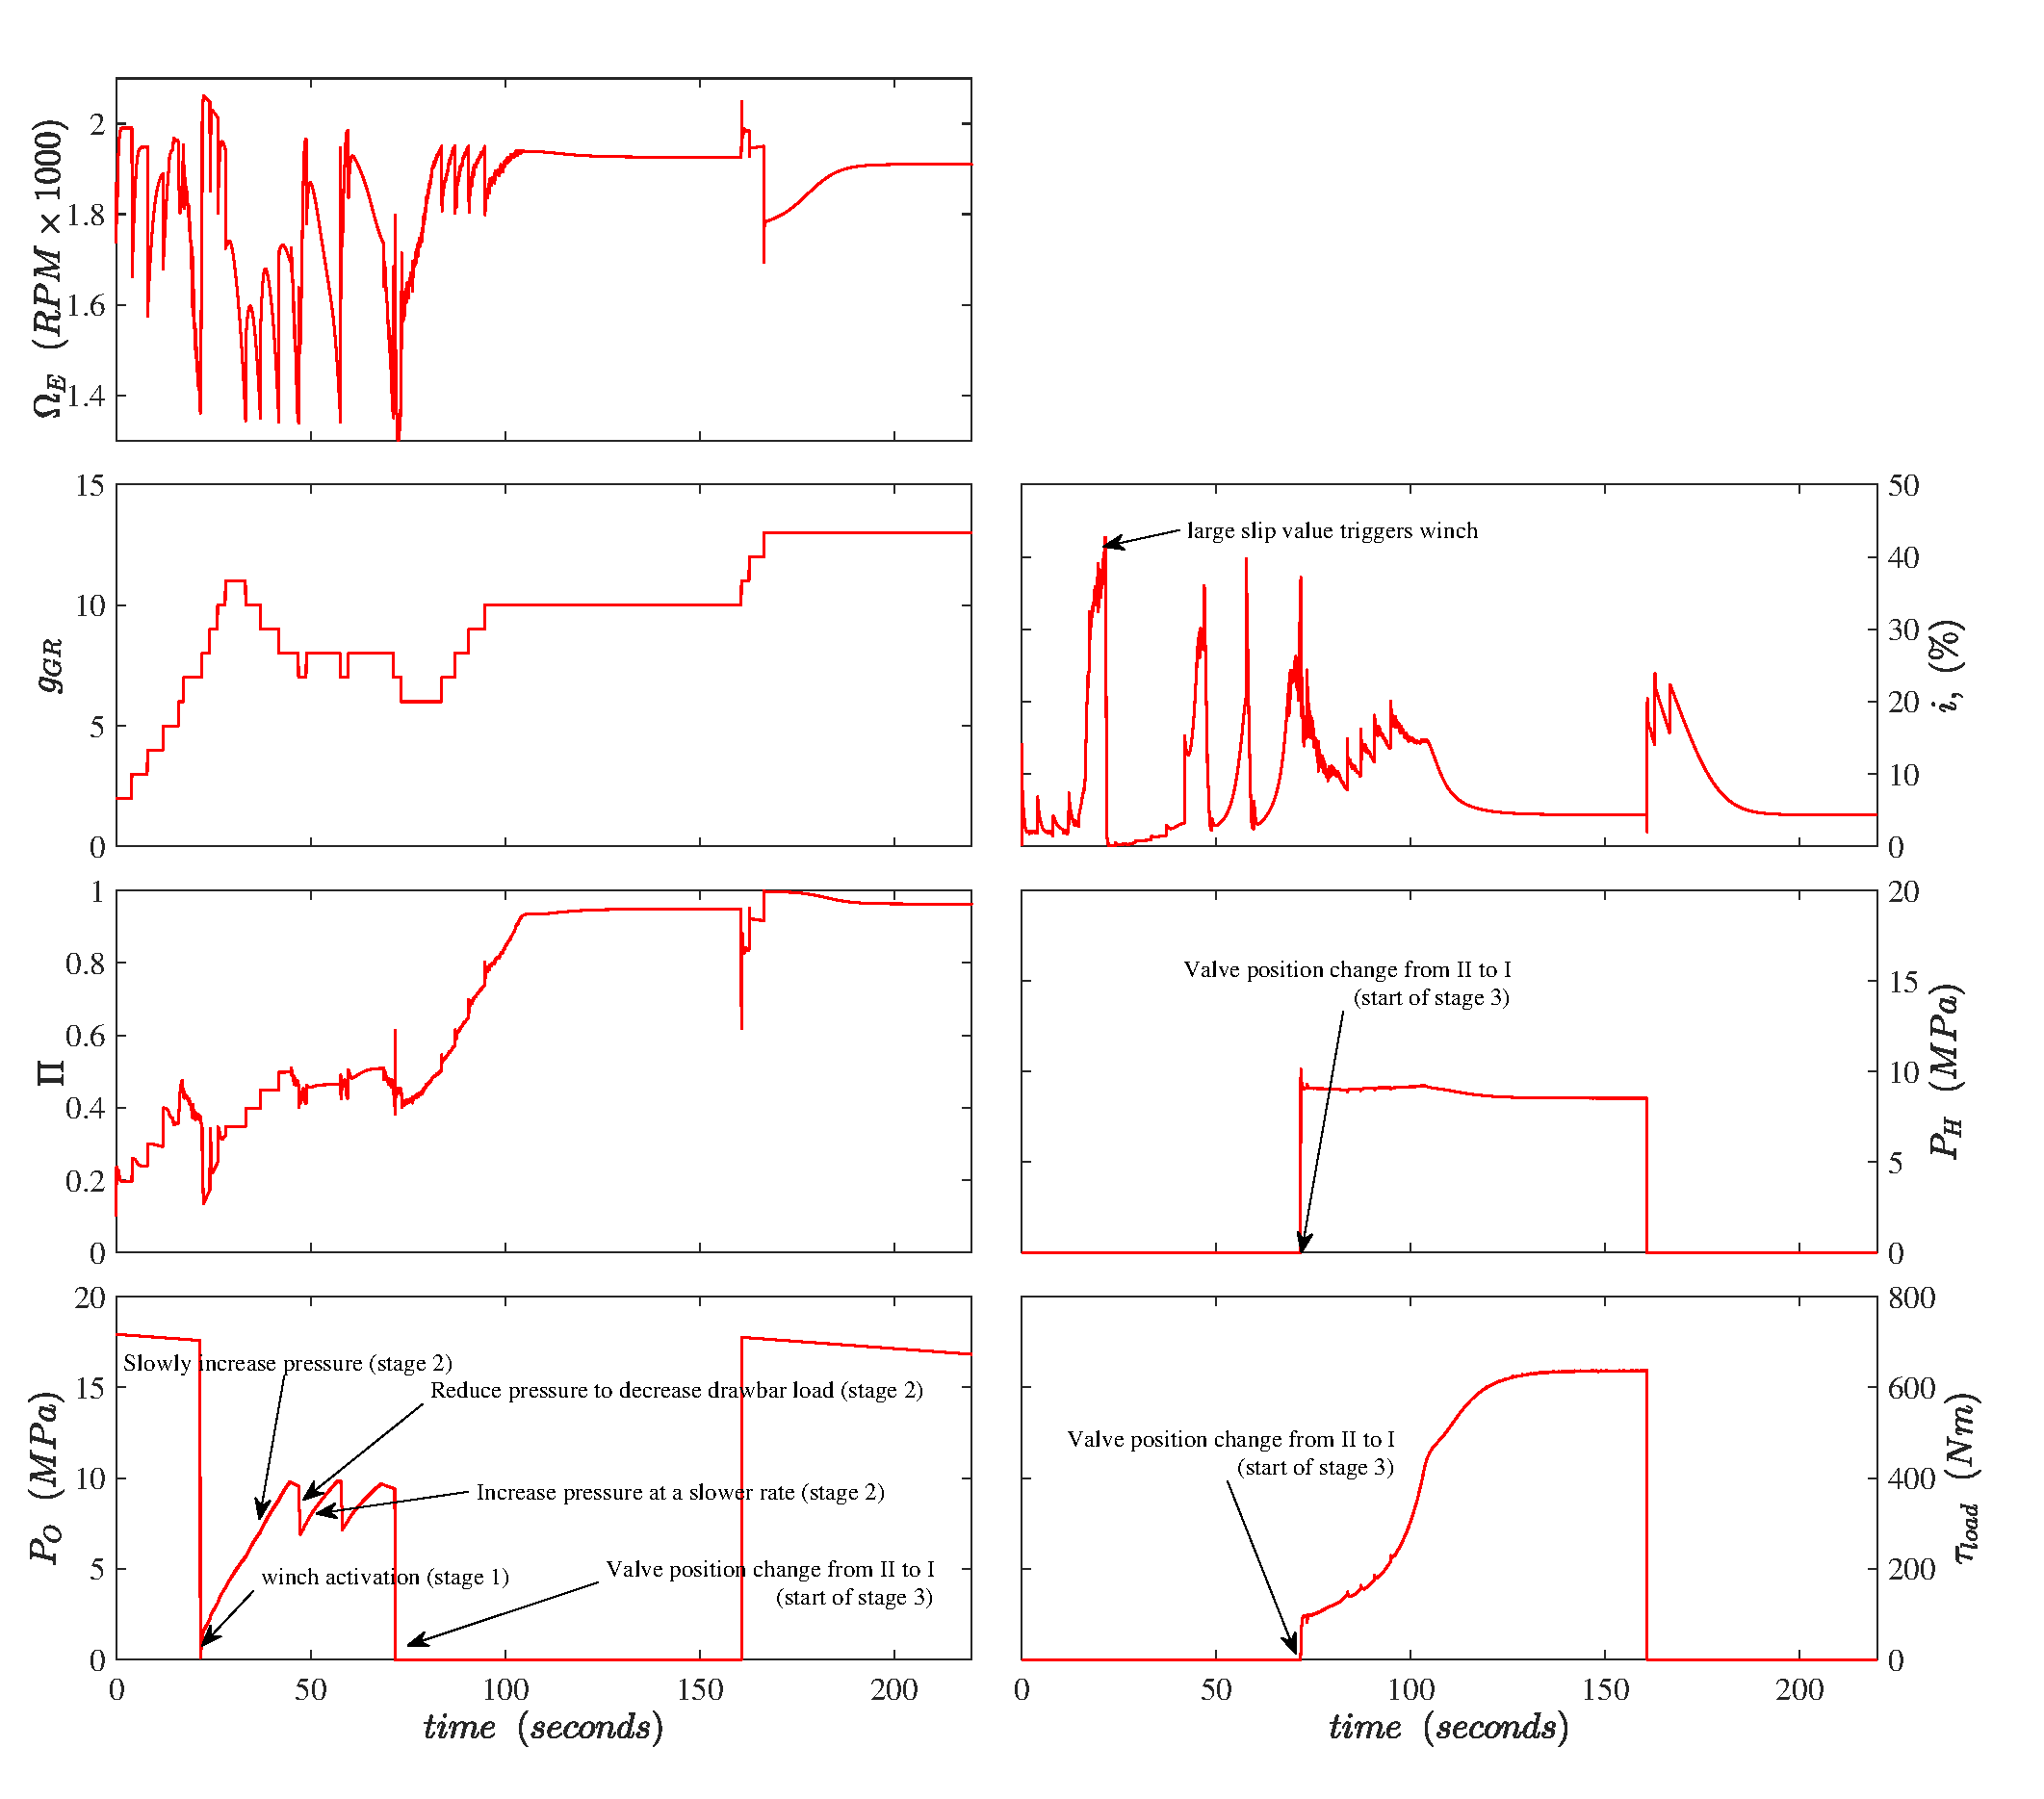
\includegraphics[width = 6in, keepaspectratio]{WC_RedTractor_Traj1}
    \caption{Plots of inputs and state variables for the red tractor using both the traction control mode and winch control mode. These include throttle and gear selection inputs $\Pi$ and $g_{GR}$ and state variables of engine speed $\Omega_E$, slip $i$, pressure of the H and O nodes in the winch hydraulics $P_H$ and $P_O$ and the load placed on the engine from the winch hydralics $\tau_{load}$.}
    \label{fig:WC_RedTractor_Traj1}
\end{figure}
\begin{figure}[p]
    \centering
    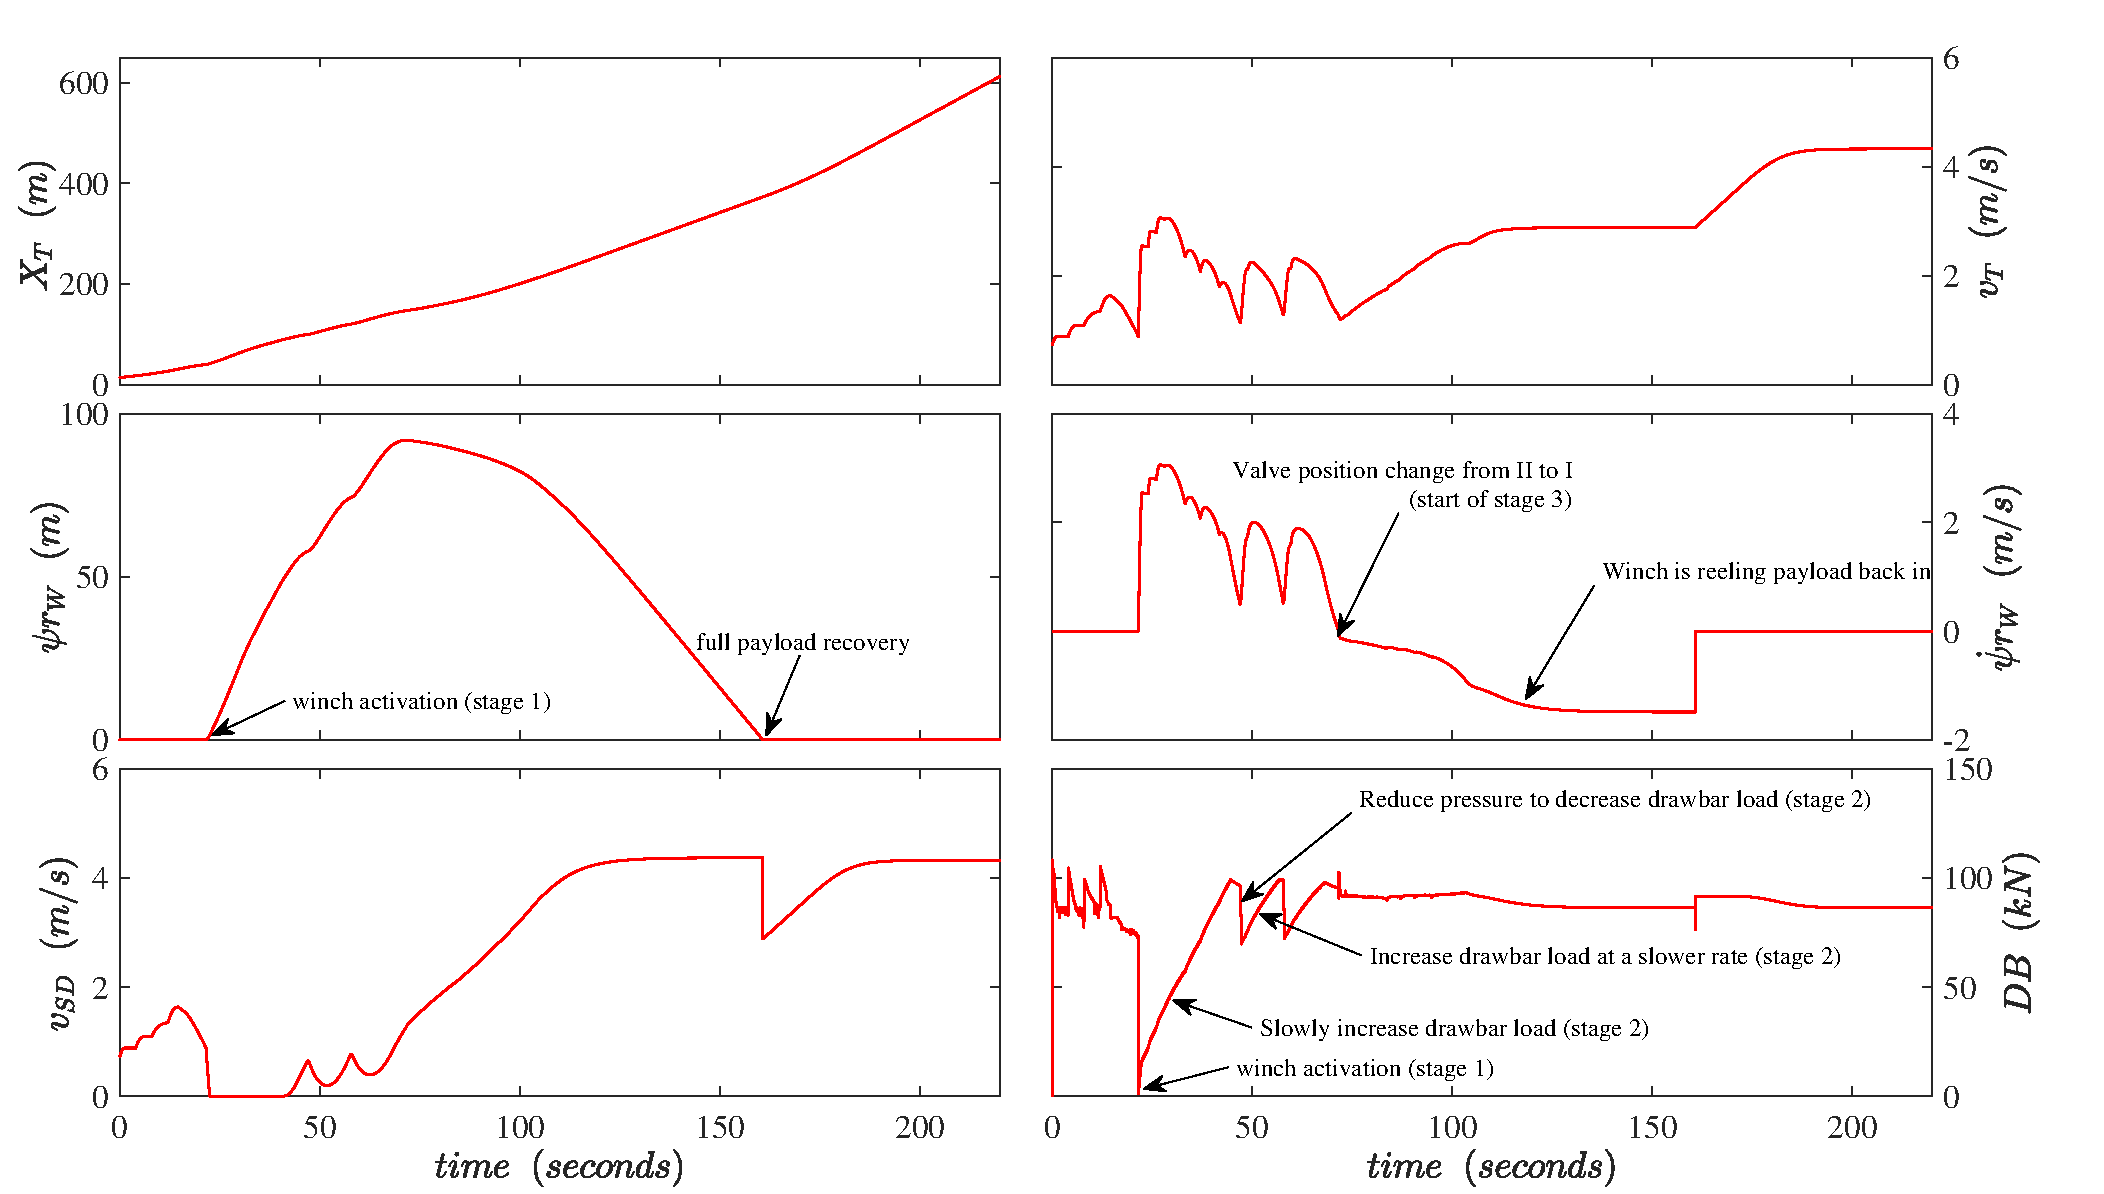
\includegraphics[width = 6in, keepaspectratio]{WC_RedTractor_Traj2}
    \caption{Plots of state variables for the red tractor using both the traction control mode and winch control mode. These include the tractors east position $X_T$, tractor speed $v_T$, cable length released $\psi r_W$, the speed of cable length be released or being pulled in $\dot{\psi} r_W$, sled speed $v_{SD}$ and drawbar load $DB$.}
    \label{fig:WC_RedTractor_Traj2}
\end{figure}
